\ifdefined\maindocument
\else
    \documentclass{article}
    \input{packages.tex}

\title{Supplemental Material for\\ ``High-threshold and low-overhead fault-tolerant quantum memory''}

 \author[1]{Sergey~Bravyi}
 \author[1]{Andrew~W.~Cross}
 \author[1]{Jay~M.~Gambetta}
  \author[1]{Dmitri~Maslov}
 \author[2]{Patrick~Rall}
 \author[1]{Theodore~J.~Yoder} 
 \affil[1]{\large{IBM Quantum, IBM T.J. Watson Research Center, Yorktown Heights, NY 10598 (USA)}}
 \affil[2]{IBM Quantum, MIT-IBM Watson AI Lab, Cambridge, MA 02142 (USA)}

    \begin{document}
    \maketitle
    
    \tableofcontents
    
   \newcommand{\figlayout}{1 }
   \newcommand{\figwheelextraction}{4 }
   \newcommand{\eqnAB}{1}
   \newcommand{\lemkd}{1 }
   \newcommand{\figsyndromecircuit}{2 }
   \newcommand{\figsmallldpc}{3 A) }
   \newcommand{\figldpcvssurface}{3 B) }
   \newcommand{\tabcodesintro}{1 }
   \newcommand{\tabcodes}{2 }
   \newcommand{\fignavigation}{5 }
   \newcommand{\lemconnected}{3 }


\fi

\newcommand{\ifmain}[2]{\ifdefined\maindocument#1\else#2\fi}

% Use this to highlight edits
%\newcommand{\edit}[1]{{\color{red}{#1}}}


\section{Syndrome measurement circuit}
\label{sec:syndrome_circuit}

The next step is to furnish the code $\qc$ with a syndrome measurement (SM) circuit that repeatedly measures the syndrome of each check operator.  Here we describe a SM circuit that requires $2n$ physical qubits in total: $n$ data qubits and $n$ ancillary check qubits used to record the measured syndromes.  The circuit only applies $\cnotgate$s to pairs of qubits that are connected in the Tanner graph. 

The SM circuit is defined as a periodically repeated sequence of {\em syndrome cycles} (SC).  A single SC is responsible for measuring syndromes of all $n$ check operators of the code.  Let $N_c$ be the number of syndrome cycles. We envision that $N_c\,{>}\,1$.  The circuit begins and ends with a special initialization and measurement cycle responsible for initializing logical qubits in a suitable initial state and measuring logical qubits in a suitable basis.  Here we focus on the optimization of the SC circuit.  Logical initialization and measurements are discussed in \sec{logicals}.


The SC circuit is divided into $N_r$ {\em rounds} such that each round is a depth-1 circuit composed of $\cnotgate$s and single-qubit operations.  The latter include initializing a qubit in the $X$ or $Z$ basis and measuring a qubit in the $X$ or $Z$ basis.  $\cnotgate$s can be applied only to pairs of qubits which are nearest neighbors in the Tanner graph.  Some qubits remain idle during some rounds, although we try to minimize such occurrences by squeezing more useful computations in as little time as possible.  Our notations are summarized in \tab{tab3}.
% By definition, a single syndrome cycle has depth $N_r$.


\begin{table}[t]
\begin{center}
\begin{tabular}{c|c}
\hline
Notation & Operation  \\
\hline
\hline
$\cnot{c}{t}$  & $\cnotgate$ with control qubit $c$ and target qubit $t$ \\
\hline
$\initX{q}$  & Initialize qubit $q$ in the state $|+\ra=(|0\ra+|1\ra)/\sqrt{2}$\\
\hline
$\initZ{q}$ &  Initialize qubit $q$ in the state $|0\ra$\\
\hline
$\measX{q}$ & Measure qubit $q$ in the $X$-basis $|+\ra,|-\ra$\\
\hline
$\measZ{q}$ & Measure qubit $q$ in the $Z$-basis $|0\ra,|1\ra$\\
\hline
$\idle{q}$ & Identity gate on qubit $q$  \\ 
\hline
\end{tabular}
\caption{Elementary operations used for syndrome measurements.}
\label{table:tab3}
\end{center}
\end{table}


\begin{table}[ht]
\begin{center}
\begin{tabular}{c|c||c|c}
\hline
Round  & Circuit & Round    & Circuit \\
\hline
\hline
1 & 
{\centering
\begin{minipage}{7cm}
	\begin{algorithmic}
	\State{}
	\For{$i=1$ to $n/2$}
	\State{$\initX{q(X,i)}$}
	\State{$\cnot{q(R,A_1^T(i))}{q(Z,i)}$}
	\State{$\idle{q(L,i)}$}
	\EndFor
	\State{}
	\end{algorithmic}
\end{minipage}}
&  5 &
{\centering
\begin{minipage}{7cm}
	\begin{algorithmic}
	\State{}
	\For{$i=1$ to $n/2$}
	\State{$\cnot{q(X,i)}{q(R,B_3(i))}$}
	\State{$\cnot{q(L,B_3^T(i))}{q(Z,i)}$}
	\EndFor
	\State{}
	\end{algorithmic}
\end{minipage}}
 \\
\hline
2 & 
{\centering
\begin{minipage}{7cm}
	\begin{algorithmic}
	\State{}
	\For{$i=1$ to $n/2$}
	\State{$\cnot{q(X,i)}{q(L,A_2(i))}$}
	\State{$\cnot{q(R,A_3^T(i))}{q(Z,i)}$}
	\EndFor
	\State{}
	\end{algorithmic}
\end{minipage}}
& 6 & 
{\centering
\begin{minipage}{7cm}
	\begin{algorithmic}
	\State{}
	\For{$i=1$ to $n/2$}
	\State{$\cnot{q(X,i)}{q(L,A_1(i))}$}
	\State{$\cnot{q(R,A_2^T(i))}{q(Z,i)}$}
	\EndFor
	\State{}
	\end{algorithmic}
\end{minipage}}
\\
\hline
3 & 
{\centering
\begin{minipage}{7cm}
	\begin{algorithmic}
	\State{}
	\For{$i=1$ to $n/2$}
	\State{$\cnot{q(X,i)}{q(R,B_2(i))}$}
	\State{$\cnot{q(L,B_1^T(i))}{q(Z,i)}$}
	\EndFor
	\State{}
	\end{algorithmic}
\end{minipage}}
& 7 &
{\centering
\begin{minipage}{7cm}
	\begin{algorithmic}
	\State{}
	\For{$i=1$ to $n/2$}
	\State{$\cnot{q(X,i)}{q(L,A_3(i))}$}
	\State{$\measZ{q(Z,i)}$}
	\State{$\idle{q(R,i)}$}
	\EndFor
	\State{}
	\end{algorithmic}
\end{minipage}}
 \\
\hline
4 & 
{\centering
\begin{minipage}{7cm}
	\begin{algorithmic}
	\State{}
	\For{$i=1$ to $n/2$}
	\State{$\cnot{q(X,i)}{q(R,B_1(i))}$}
	\State{$\cnot{q(L,B_2^T(i))}{q(Z,i)}$}
	\EndFor
	\State{}
	\end{algorithmic}
\end{minipage}}
& 8 & 
{\centering
\begin{minipage}{7cm}
	\begin{algorithmic}
	\State{}
	\For{$i=1$ to $n/2$}
	\State{$\measX{q(X,i)}$}
	\State{$\initZ{q(Z,i)}$}
	\State{$\idle{q(L,i)}$}
	\State{$\idle{q(R,i)}$}
	\EndFor
	\State{}
	\end{algorithmic}
\end{minipage}}
\\
\hline
\end{tabular}
\end{center}
\caption{Depth-8 syndrome measurement cycle circuit.}
\label{table:syndromecircuit}
\end{table}



Below we describe a SC circuit with effectively $N_r\,{=}\,8$ rounds\footnote{The operator $\initZ{q(Z,i)}$ must be executed before the first application of this SC circuit, raising the depth of the first stage to 9.  However, each following syndrome cycle takes Z-check initialization from the previous round. Last syndrome cycle needs not apply the Z-check state initialization.  Total SM circuit depth with $N_c$ syndrome cycles is thus $8N_c\,{+}\,1$.}.  Ignoring single-qubit initialization and measurement operations, the SC circuit is a depth-7 $\cnotgate$ circuit.  By designing the circuit for an explicit family of LDPC codes we are able to leverage the symmetries and reduce computational depth to $7$ from what otherwise would be $14\,{=}\,2{\cdot}6\,{+}\,2$, as shown by previous authors \cite[Theorem 1]{tremblay2022constant}.  Our notations are as follows.  We divide $n$ data qubits into the left and the right registers $q(L)$ and $q(R)$ of size $n/2$ each.  Each check operator acts on three data qubits from $q(L)$ and three data qubits from $q(R)$.  The SM circuit uses $2n$ physical qubits in total: $n$ data qubits and $n$ ancillary check qubits that record  the syndrome of each check operator.  Let $q(X)$ and $q(Z)$ be the ancillary registers of size $n/2$ that span $X$-check and $Z$-check qubits respectively.
Thus the physical qubits are partitioned into four registers,  $q(X)$, $q(L)$, $q(R)$, and $q(Z)$, of size $n/2$ each. Label qubits in each register by integers $i=1,2,\ldots,n/2$.
We write $q(X,i)$ for the $i$-th qubit of the register $q(X)$ with similar notations for $q(L)$, $q(R)$, and $q(Z)$.
Each permutation matrix $A_p$ and $B_q$ from \ifmain{Eq.~(\ref{AB})}{Eq.~(\eqnAB) in the main text} defines a one-to-one map from the set $\{1,2,\ldots,n/2\}$ onto itself.

We identify a permutation matrix and the corresponding one-to-one map. For example, we write $j\,{=}\,A_1(i)$ if the matrix $A_1$ has a one at row $i$ and column $j$ (this is well defined since $A_1$ is a permutation matrix).
Likewise, we write $j\,{=}\,A_1^T(i)$ if the transposed matrix $A_1^T$ has a one at the row $i$ and column $j$.
In this notation, the $i$-th $X$-check operator acts on data qubits $q(L,A_p(i))$ and $q(R,B_p(i))$ with $p=1,2,3$.  The $i$-th $Z$-check operator acts on data qubits $q(L,B_p^T(i))$ and $q(R,A_p^T(i))$ with $p=1,2,3$.


\ifdefined\maindocument
\begin{figure}[t]
  \centering
    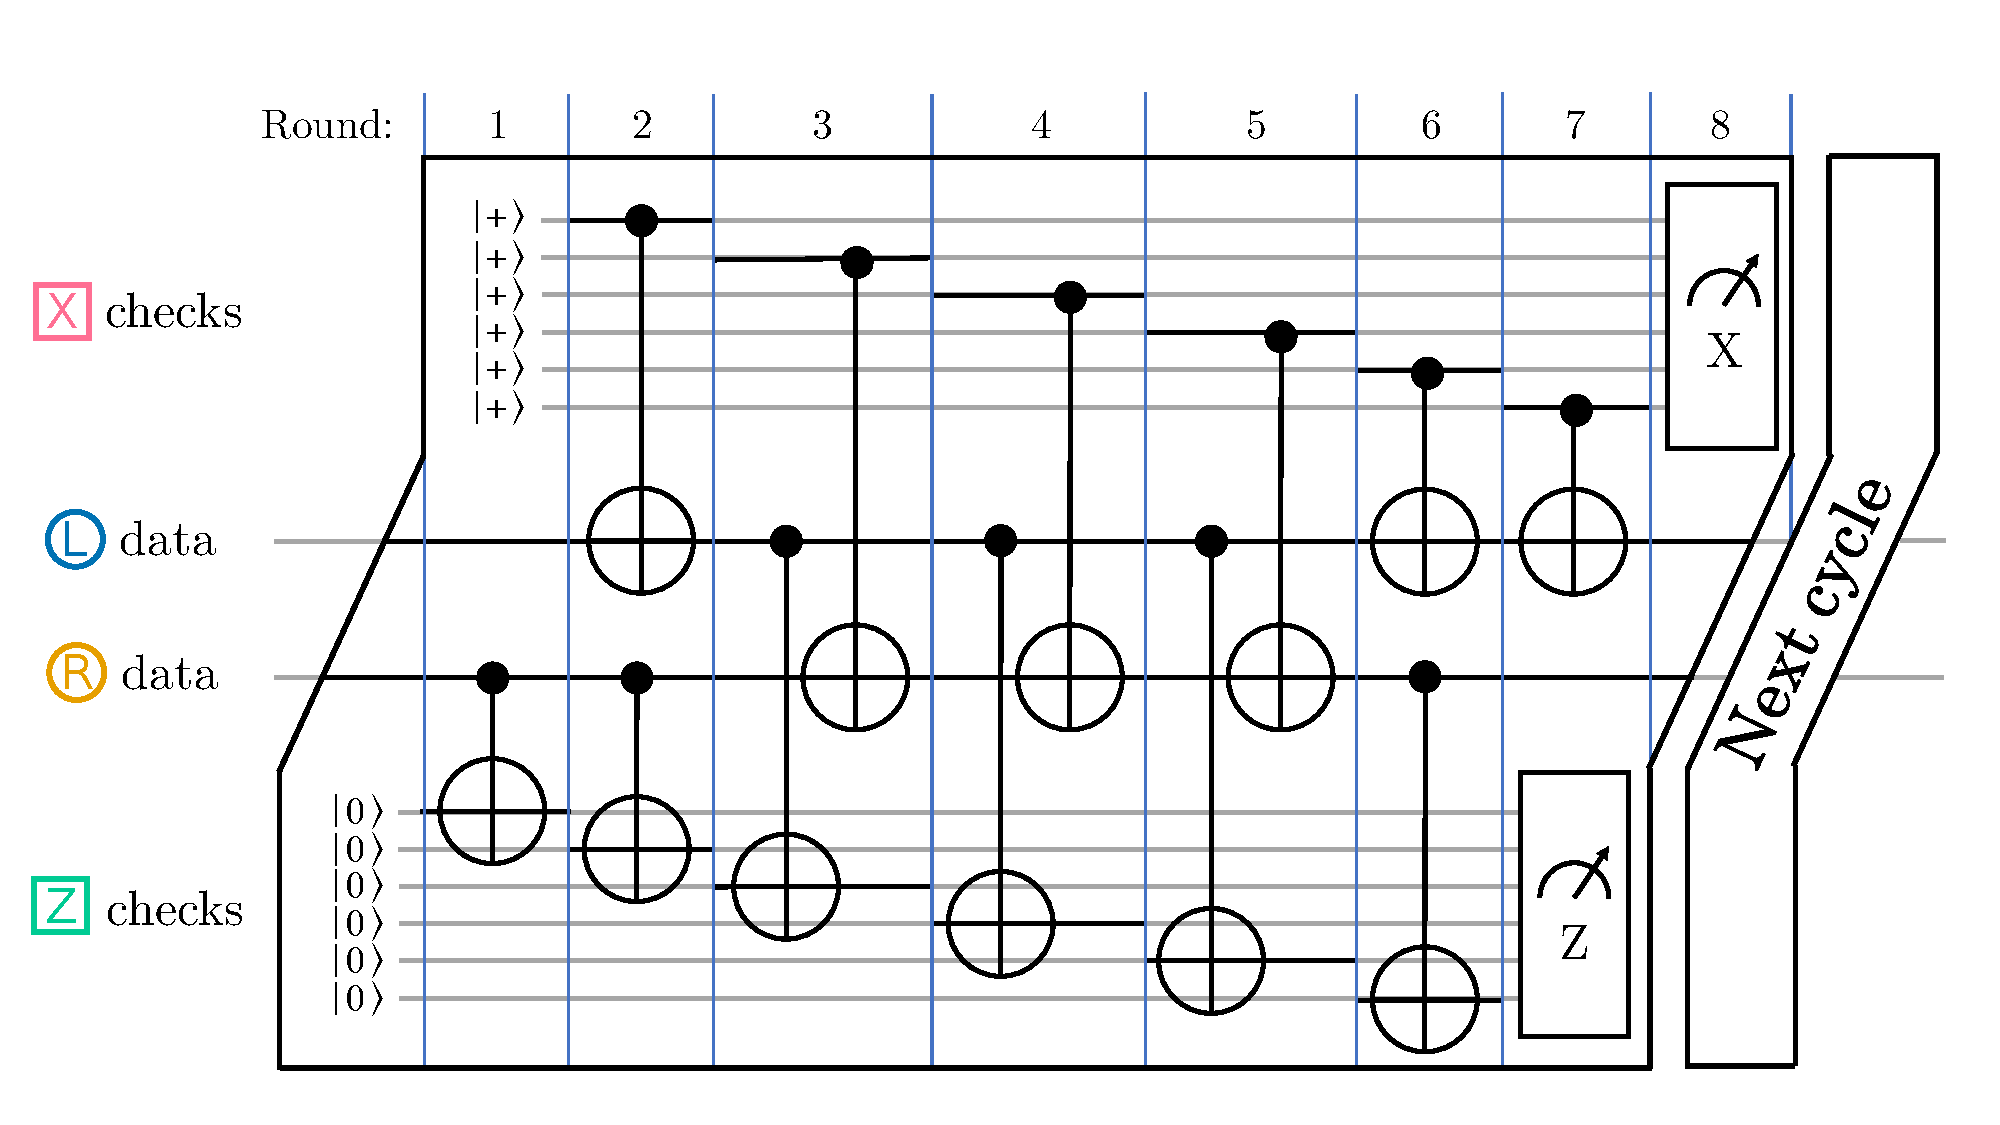
\includegraphics[height=8cm]{syndromecircuit.pdf}
     \caption{Depth-8 syndrome measurement cycle circuit.}
  \label{fig:syndromecircuit}
\end{figure}
\else
\fi

Our depth-8 SC circuit is described in \tab{syndromecircuit} and illustrated in \ifmain{\fig{syndromecircuit}}{Figure~\figsyndromecircuit in the main text}.  Note that within each round all operations act over non-overlapping sets of qubits.  In particular, each round applies at most one layer of $\cnotgate$ gates between $q(X)$ and $q(L)$ registers (Rounds 2, 6, and 7), at most one layer of $\cnotgate$s between $q(X)$ and $q(R)$ registers (Rounds 3, 4, and 5), at most one layer of $\cnotgate$s between $q(Z)$ and $q(L)$ registers (Rounds 3, 4, and 5), and at most one layer of $\cnotgate$s between $q(Z)$ and $q(R)$ registers (Rounds 1, 2, and 6). Qubits from $q(Z)$ are always targets for $\cnotgate$s.  Accordingly, $X$-type errors propagate from data qubits to check qubits in $q(Z)$.  The latter are measured in the $Z$-basis in Round 7 revealing the syndrome of $X$-type errors. Qubits from $q(X)$ are always controls for $\cnotgate$s. Accordingly, $Z$-type errors propagate from data qubits to check qubits in $q(X)$.  The latter are measured in the $X$-basis in Round~8 revealing the syndrome of $Z$-type errors.  We envision that the syndrome cycles are repeated periodically. This justifies applying $\cnotgate$s to $q(Z)$ at Round~1 even though $q(Z)$ is initialized only at Round~8.  Indeed, Round~8 of the previous syndrome cycle goes immediately before Round~1 of the current cycle. Thus $q(Z)$ has been already initialized at the beginning of Round~1.  We were not able to find a depth-8 (or smaller depth) syndrome cycle in which $X$-check and $Z$-check qubits are initialized and measured synchronously. 

Let us now prove that the above SC circuit has the desired functionality.  Since the circuit involves only Clifford operations, its action can be compactly described using stabilizer tableau~\cite{aaronson2004improved}.  We track how the tableau changes as each layer of $\cnotgate$s in the circuit is applied.  Since the $\cnotgate$ gates do not mix Pauli $X$ and $Z$ operators, one may consider tableau describing the action of the circuit on $X$-type and $Z$-type Pauli operators separately.  

Let us begin with $X$-type Pauli.  The corresponding tableau $T$ is a binary matrix of size $n\,{\times}\, 2n$ such that each row of $T$ defines an $X$-type stabilizer of the underlying quantum state.  We partition columns of $T$ into four blocks that represent qubit registers $q(X)$, $q(L)$, $q(R)$, and $q(Z)$.  We partition rows of $T$ into two blocks such that initially the top $n/2$ rows represent weight-$1$ check operators on qubits of the register $q(X)$ initialized in the state $|+\ra$ while the bottom $n/2$ rows represent weight-$6$ check operators on data qubits associated with the chosen code $\qc$. 
Thus, at the beginning of Round~1, when all check qubits in the register $q(X)$ have been initialized in the state $|+\ra$, while data qubits are in some logical state of the code $\qc$, the binary matrix is 
\[
\begin{pmatrix}
I & 0 & 0 & 0 \\
0 & A & B & 0
\end{pmatrix}.
\]
Here $I\,{\equiv}\, I_{n/2}$ is the identity matrix. 
The SC circuit (ignoring qubit initialization and measurements) enacts the transformation
\[
\begin{pmatrix}
I & 0 & 0 & 0 \\
0 & A & B & 0
\end{pmatrix}
\xrightarrow{\text{SC circuit}}
\begin{pmatrix}
I & A & B & 0 \\
0 & A & B & 0 
\end{pmatrix}.
\]
Indeed, the circuit must map a single-qubit $X$ stabilizer $X_j$ on a check qubit $j\,{\in}\, q(X)$ to a product of $X_j$ and the $j$-th $X$-type check operator on the data qubits determined by the $j$-th row of $H^X=[A|B]$.
The eigenvalue measurement of $X_j$ at the final round then reveals the syndrome of the $j$-th check operator.
The bottom $n/2$ rows must be unchanged since the check operators of the code must be the same before and after the syndrome measurement.

Let us verify that the circuit defined in \tab{syndromecircuit} enacts the desired transformation. To accomplish this, we rewrite the SC circuit by removing notations irrelevant to showing the correctness of $X$-checks.  Specifically, we write each $\cnotgate$ in \tab{syndromecircuit} as $\cnotgate_M(a,b)$, where $a,b \,{\in}\, \{1, 2, 3, 4\} = \{q(X), q(L), q(R), q(Z)\}$, and $M \,{\in}\, \{A_1,A_2,A_3,B_1,B_2, B_3\}$. Note that the $\cnotgate$ instructions where the matrix $M^T$ is used instead of $M$ can be written using matrix $M$ by performing the variable renaming $i\,{\gets}\, M(i)$ in the corresponding for loop in \tab{syndromecircuit}.

Using the above compact notation, the unitary part of the SC circuit becomes:
\be
\ba{cc}
\text{Round~1:} & \hfill \cnotgate_{A_1}(3,4) \\
\text{Round~2:} & \cnotgate_{A_2}(1,2), \cnotgate_{A_3}(3,4) \\
\text{Round~3:} & \cnotgate_{B_2}(1,3), \cnotgate_{B_1}(2,4) \\
\text{Round~4:} & \cnotgate_{B_1}(1,3), \cnotgate_{B_2}(2,4) \\
\text{Round~5:} & \cnotgate_{B_3}(1,3), \cnotgate_{B_3}(2,4) \\
\text{Round~6:} & \cnotgate_{A_1}(1,2), \cnotgate_{A_2}(3,4) \\
\text{Round~7:} & \cnotgate_{A_3}(1,2) \hfill \\
\ea
\label{SCunitary_part}
\ee


In the following we apply all seven unitary rounds to verify the correctness of the performed transformation:
\[
\text{Round~1:}
\begin{pmatrix}
I & 0 & 0 & 0 \\
0 & A & B & 0
\end{pmatrix}
\xrightarrow{\cnotgate_{A_1}(3,4)}
\begin{pmatrix}
I & 0 & 0 & 0 \\
0 & A & B & A_1 B
\end{pmatrix}
\]

\[
\text{Round~2:}
\xrightarrow{\cnotgate_{A_2}(1,2)}
\begin{pmatrix}
I & A_2 & 0 & 0 \\
0 & A & B & A_1 B
\end{pmatrix}
\xrightarrow{\cnotgate_{A_3}(3,4)}
\begin{pmatrix}
I & A_2 & 0 & 0 \\
0 & A & B & (A_1{+}A_3)B \\
\end{pmatrix}
\]

\[
\text{Round~3:}
\xrightarrow{\cnotgate_{B_2}(1,3)}
\begin{pmatrix}
I & A_2 & B_2 & 0 \\
0 & A & B & (A_1{+}A_3)B
\end{pmatrix}
\xrightarrow{\cnotgate_{B_1}(2,4)}
\begin{pmatrix}
I & A_2 & B_2 & A_2B_1 \\
0 & A & B & (A_1{+}A_3)B+AB_1 \\
\end{pmatrix}
\]

\[
\text{Round~4:}
\xrightarrow{\cnotgate_{B_1}(1,3)}
\begin{pmatrix}
I & A_2 & B_1{+}B_2 & A_2 B_1 \\
0 & A & B & (A_1{+}A_3)B + AB_1 \\
\end{pmatrix}
\]
\[
\xrightarrow{\cnotgate_{B_2}(2,4)}
\begin{pmatrix}
I & A_2 & B_1{+}B_2 & A_2 (B_1{+}B_2) \\
0 & A & B & (A_1{+}A_3)B+A(B_1{+}B_2) \\
\end{pmatrix}
=
\begin{pmatrix}
I & A_2 & B_1{+}B_2 & A_2 (B_1{+}B_2) \\
0 & A & B & A_2B + AB_3 \\
\end{pmatrix}
\]
Here, we use the identity $(A_1{+}A_3)B+A(B_1{+}B_2)=A_2B + AB_3$, which holds since the sum of first summands and second summands on both sides of the equation gives $AB$, and $AB\,{+}\,AB\,{=}\,0$.

\[
\text{Round~5:}
\xrightarrow{\cnotgate_{B_3}(1,3)}
\begin{pmatrix}
I & A_2 & B & A_2 (B_1{+}B_2) \\
0 & A & B & A_2B + AB_3  \\
\end{pmatrix}
\xrightarrow{\cnotgate_{B_3}(2,4)}
\begin{pmatrix}
I & A_2 & B & A_2 B \\
0 & A & B & A_2B   \\
\end{pmatrix}
\]

\[
\text{Round~6:}
\xrightarrow{\cnotgate_{A_1}(1,2)}
\begin{pmatrix}
I & A_1{+}A_2 & B & A_2 B \\
0 & A & B & A_2B   \\
\end{pmatrix}
\xrightarrow{\cnotgate_{A_2}(3,4)}
\begin{pmatrix}
I & A_1{+}A_2 & B & 0 \\
0 & A & B & 0  \\
\end{pmatrix}
\]

\[
\text{Round~7:}
\xrightarrow{\cnotgate_{A_3}(1,2)}
\begin{pmatrix}
I & A & B & 0 \\
0 & A & B & 0  \\
\end{pmatrix}.
\]

\noindent This is the desired transformation.

So far, we have not considered the action of the SC circuit on the logical qubits of the code.  Let us show that this action is trivial.  Indeed, consider some $X$-type logical operator $X(v)$, where $v\,{\in}\, \FF_2^n$. Write $v\,{=}\,(u,w)$ where $u$ and $w$ are restrictions of $v$ onto the registers 2 and 3 respectively. Commutativity between $X(v)$ and any $Z$-type check operator implies 
\[
uB+wA=0.
\]
Here we consider $u$ and $w$ as row vectors.  Extending $v$ by zeroes on registers 1 and 4 gives the row vector $(0\; u \; w\; 0)$, where $0$ stands for the all-zero row vector of length $n/2$.  Let us follow the same chain of transformations as above starting from the initial vector $(0\; u \; w\; 0)$. All $\cnotgate$s controlled by the register 1, such as $\cnotgate_{A_2}(1,2)$ or $\cnotgate_{B_2}(1,3)$ in Eq.~(\ref{SCunitary_part}), have trivial action on the vector $(0\; u \; w\; 0)$ since all qubits of the control register are zeroes.  Such $\cnotgate$s can be omitted.  The remaining $\cnotgate$s in Eq.~(\ref{SCunitary_part}) such as $\cnotgate_{A_1}(3,4)$ or $\cnotgate_{B_1}(2,4)$ map the initial vector $(0\; u \; w\; 0)$ to $(0\; u \; w\; t)$ for some vector $t$ since the registers 2 and 3 always serve as the controls and the register 4 always serves as the target.  Rounds~1, 2, and 6 in Eq.~(\ref{SCunitary_part})  are equivalent to XORing vectors $wA_1$, $wA_3$, and $wA_2$ respectively to the register 4.  Rounds~3, 4, and 5 in Eq.~(\ref{SCunitary_part}) are equivalent to XORing vectors $uB_1$, $uB_2$, and $uB_3$ respectively to the register 4.  Thus
\[
t = w(A_1{+}A_2{+}A_3) + u(B_1{+}B_2{+}B_3) = wA + uB = 0.
\]
We have shown that the SC circuit maps the vector  $(0\; u \; w\; 0)$ to itself. Hence the circuit acts trivially on logical $X$-type operators. 

To prove the correctness of $Z$-checks, observe that $Z$-checks can be mapped into $X$-checks by conjugation with Hadamards.  When the unitary circuit in \ifmain{\fig{syndromecircuit}}{Figure~\figsyndromecircuit in the main text} is conjugated with Hadamards, this flips controls and targets of all $\cnotgate$ gates.  Thus, to verify $Z$-checks, it suffices to perform a very similar calculation to the one already shown for $X$-checks.  We omit this calculation here.

%{\color{red} THIS PARAGRAPH NEEDS TO BE REWRITTEN: The randomized noisy simulations of our SM circuit suggest that the logical error probability per syndrome cycle scales as $p_L\sim p^{d/2}$ for small error rates $p$, see Figure~\ref{fig:small_ldpc}. Thus we conjecture that this circuit is distance-preserving.  This conjecture is further supported by estimating the minimum number of faulty operations resulting in a logical error using BP-OSD method, as detailed in Section~\ref{sec:decoder}.  The short depth of the single cycle, relying on only seven computational stages, also helps to keep the spread of errors under control.}

The SC circuit shown in \tab{syndromecircuit} is not unique in the following sense: we found 935 depth-7 alternatives to the unitary part of the SC circuit via a computer search. 
%SBB: there are much more than 935  alternatives unless we restrict each layer of gates to be cnot_{A_i} or cnot_{B_j}
These alternatives are obtained from the circuit defined in  Eq.~(\ref{SCunitary_part}) by applying the gate layers $\cnotgate_{A_i}$ and $\cnotgate_{B_j}$ in a different order. 
In the special case of the $[[144,12,12]]$ code,
numerical simulations show that all 936 variants of the syndrome cycle give rise to syndrome measurement circuits with distance $\dcirc\le 10$ explaining our focus on a specific circuit Eq.~(\ref{SCunitary_part}) which we conjecture to have distance $\dcirc\,{=}\,10$.  The short depth of the single cycle, relying on only seven computational stages, helps to keep the spread of errors under control.  Details of calculating upper bounds on the circuit-level distance are provided in \sec{decoder}.




\section{Decoder for the circuit-based noise model}
\label{sec:decoder}


So far we assumed that  the SM circuit is noiseless.
As shown in \sec{syndrome_circuit},
in this case all measured syndromes are zero and the circuit implements the logical identity gate.
Consider now what happens when each operation in the circuit including $\cnotgate$ gates, qubit initializations,
measurements, and idle qubits is subject to noise. To enable efficient decoding and
numerical simulations, we use
the standard circuit-based depolarizing noise model~\cite{fowler2009high}.
It assumes that each operation in the circuit is  ideal or faulty with the
probability $1-p$ or $p$ respectively. Here $p$ is a model parameter
called the error rate. Faults on different operations occur independently.
We define faulty operations as follows.
A faulty $\cnotgate$  is an ideal $\cnotgate$
followed by one of $15$ non-identity Pauli errors on the control and the target qubits
 picked uniformly at random. A faulty initialization
prepares a single-qubit state orthogonal to the correct one.
A faulty measurement is an ideal measurement followed by a classical
bit-flip error applied to the measurement outcome.
A faulty idle  qubit suffers from a Pauli error
$X$ or $Y$ or $Z$ picked uniformly at random.

To perform error correction one needs a decoder — a classical algorithm that takes as input
the measured  error syndrome and outputs a guess of the final Pauli error on the data qubits resulting from all
faults in the SM circuit. The error syndrome may itself be faulty
due to measurement errors. The decoder succeeds if the guessed Pauli error 
coincides with the actual error up to  a product of check operators.
In this case the guessed and the actual error have the same action on any logical state.


Let us show how to adapt Belief Propagation with an Ordered Statistics 
postprocessing step
Decoder (BP-OSD) proposed in~\cite{panteleev2021degenerate,roffe2020decoding}
to the circuit-based noise model.
The decoder consists of two stages.
The first stage takes as input a BB
code $\qc$ equipped with a SM circuit $\calU$  and an error rate $p$. 
It outputs a certain linearized noise model 
that ignores possible cancellations between errors generated by two or more faulty
operations in $\calU$.  This stage is analogous to computing
the decoding graph in error correction algorithms based on the surface code~\cite{fowler2012topological,higgott2023sparse}.
The second (online) stage of the decoder
 takes as input an
error syndrome measured in the experiment
and outputs a guess of the final error on the data qubits. 
This stage
 decodes the linearized noise model
using BP-OSD method~\cite{panteleev2021degenerate,roffe2020decoding}.
\edit{Our linearized noise model is conceptually similar to 
spacetime codes studied by Delfosse and Paetznick~\cite{delfosse2023spacetime}
and detector-based noise model proposed
by McEwen, Bacon, and Gidney~\cite{mcewen2023relaxing}. The online stage of our decoder closely follows Refs.~\cite{higgott2023improved,geher2023tangling}. In particular, Geh\'er, Crawford, and Campbell~\cite{geher2023tangling} applied BP-OSD to study tangled syndrome measurement circuits capable of measuring certain non-local check operators on a hardware with short-range
qubit connectivity.
Higgott et al~\cite{higgott2023improved} showed that the performance of the standard minimum-weight matching decoder can be enhanced by computing  prior error probabilities using BP-decoder as a preprocessing step. 
 }


We begin by describing the offline stage.
Consider a BB code  with parameters $[[n,k,d]]$ and let
$\calU$ be the SM
circuit 
constructed  in \sec{syndrome_circuit} with $N_c$ syndrome cycles.
The circuit $\calU$ contains $6nN_c$ $\cnotgate$s, $nN_c$ initializations and measurements, and $2n N_c$ idle qubit locations.
Let $\calU_1,\calU_2,\ldots,\calU_M$ be the list of all possible faulty realizations of $\calU$
with  exactly one faulty operation. If the faulty operation happens to be $\cnotgate$ or an idle qubit, 
one of the admissible Pauli errors for this operation is specified. 
A simple counting shows that $M=98nN_c$, where $98=15\cdot 6 + 1 + 1 + 3\cdot 2$
accounts for $15$ noisy realizations of each $\cnotgate$, $3$ realizations of memory errors
on idle qubits, noisy initializations and measurements.  
By definition, the list $\calU_1,\calU_2,\ldots,\calU_M$ includes all realizations of $\calU$
that can occur with the probability $O(p)$ in the limit $p\to 0$.
We simulate each circuit $\calU_j$ by propagating the chosen Pauli error towards the final time step
 taking into account qubit initialization and measurement errors (if any).
This simulation can be performed efficiently using the stabilizer formalism.
Let $s_j^U\in \{0,1\}^{nN_c}$ be the full measured syndrome of $\calU_j$ and $E_j$ be the final 
$n$-qubit Pauli error
on the data qubits generated by $\calU_j$. 
Let $s_j^F\in \{0,1\}^n$ be the syndrome of the final error $E_j$.
In other words, if we write $E_j=X(\alpha_j)Z(\beta_j)$ for some vectors $\alpha_j,\beta_j\in \{0,1\}^n$, then
\[
s_j^F= 
\left[
\ba{c}
H^Z \alpha_j \\ 
H^X \beta_j\\
\ea
\right].
\]
Here $H^X$ and $H^Z$ are the check matrices of the chosen code. 
Finally, let $s_j^L\in \{0,1\}^{2k}$ be a {\em logical syndrome} of the final error $E_j$ defined as follows.
Fix some basis set of logical Pauli operators $\overline{P}_1,\overline{P}_2,\ldots,\overline{P}_{2k}$ for the chosen code.
For example, $\overline{P}_1,\overline{P}_2,\ldots,\overline{P}_k$ could be logical $X$-type operators
and  $\overline{P}_{k+1},\overline{P}_{k+2},\ldots,\overline{P}_{2k}$ could be logical $Z$-type operators.
The $i$-th bit of $s^L_j$ is defined as 
\[
(s_j^L)_i = \left\{
\ba{rcl}
1 &\mbox{if}& E_j \overline{P}_i = -\overline{P}_i  E_j,\\
0  &\mbox{if}& E_j \overline{P}_i = \overline{P}_i  E_j,\\
\ea\right.
\]
for $i=1,\ldots,2k$. Note that the pair of syndromes $s_j^F,s_j^L$ uniquely determines the final error $E_j$
modulo check operators. Define a  pair of {\em decoding matrices} $D$ and $D^L$
of size $(nN_c+n) \times M$ and $2k\times M$ respectively
such that the $j$-th column of $D$ is
\[
\left[
\ba{c}
s^U_j  \\ 
s^F_j \\
\ea
\right]
\]
and the $j$-th column of $D^L$ is $s^L_j$.
Let $p_j$ be the probability of a Pauli error that occurred  in the circuit $\calU_j$.
We have $p_j=p/15$ if $\calU_j$ contains a faulty $\cnotgate$, 
$p_j=p/3$ if $\calU_j$ contains a faulty idle qubit,
and $p_j=p$ if $\calU_j$ contains a faulty qubit initialization or measurement.
Suppose $I \subseteq \{1,2,\ldots,M\}$ is a subset of columns of 
$D$ such that  triples of syndromes  $(s^U_j,s^F_j,s^L_j)$ are the same for all
$j\in I$. We merge all columns in $I$ to a single column 
 and assign the value
  $\sum_{j\in I} p_j$ 
to the bit-flip error probability associated with the merged column.
Let $M$ be the number of columns of $D$ after the merging step
and $p_1,p_2,\ldots,p_M$ be the respective error probabilities.

Next,  the decoding matrix $D$ is converted  to a sparse form.
To this end consider a faulty circuit $\calU_j$ and a sequence of syndromes
measured by $\calU_j$ on some check operator. Let this sequence be
$m=(m_1,m_2,\ldots,m_{N_c})\in \{0,1\}^{N_c}$. Since $\calU_j$ contains a single fault, 
the sequence $m$ has only a few locations where the measured
syndromes differ at two consecutive cycles.
For example, if $\calU_j$ contains a Pauli error on some idle data qubit between two syndrome cycles,
the $m$-sequence may look as $(0,0,\ldots,0,1,1,\ldots,1)$.
Such sequence can be made sparse if we represent it by a binary vector
\[
m'=(m_1,m_2\oplus m_1,m_3\oplus m_2,\ldots, m_{N_c}\oplus m_{N_c-1}) \in \{0,1\}^{N_c}.
\]
In other words, $m'$ stores changes in the measured syndrome at a given check operators
at each cycle. We convert the matrix $D$ to a sparse form by applying the map $m\to m'$ to the syndromes measured by each check operator for each faulty circuit $\calU_j$.

Let $\xi_1,\xi_2,\ldots,\xi_M \in \{0,1\}$ be independent random variables such that
$\xi_j$ takes values $0$ and $1$ with the probability $1-p_j$ and $p_j$
respectively.
Define a linearized noise model  that outputs a random triple $(s^U,s^F,E)$,
where
\[
E=\prod_{j=1}^M (E_j)^{\xi_j}
\]
 is an $n$-qubit Pauli error
and
\[
 \left[
\ba{c}
s^U  \\ 
s^F \\
\ea
\right]= 
\sum_{j=1}^M \xi_j  \left[
\ba{c}
s^U_j  \\ 
s^F_j \\
\ea
\right] {\pmod 2}
\]
is a binary vector that represents the error syndrome.
The linearized model is a simplified version of the circuit-based noise that
ignores possible cancellations among errors generated by two or more faulty
operations in $\calU$. Note that such errors occur with the probability only $O(p^2)$.
The decoder attempts to guess the final error $E$
acting on the data qubits
based on the syndrome $s^U$ measured in the experiment  making a simplifying assumption
that that the  pair $(s^U,E)$ was generated using the linearized noise model.
We additionally assume that the decoder
knows the syndrome $s^F$ of the final error $E$.
This syndrome can be acquired  by adding one noiseless  cycle
at the end of the syndrome measurement circuit,
which is a common practice in numerical simulations of error correction.
By definition, we have
\[
D\xi= \left[
\ba{c}
s^U  \\ 
s^F \\
\ea
\right].
\]
Here $\xi=(\xi_1,\xi_2,\ldots,\xi_M)$ is  a column vector and matrix-vector multiplication is modulo two. 
Define a minimum weight error $\xi^*=\xi^*(s)\in \{0,1\}^M$ as 
a solution of an optimization problem
\be
\label{MWD}
\xi^* = \arg \min_{\xi \in \{0,1\}^M} \; \sum_{j=1}^M \log{(1/p_j)} \xi_j \quad
\mbox{subject to} \quad 
D\xi = \left[
\ba{c}
s^U  \\ 
s^F \\
\ea
\right].
\ee
This problem is equivalent to the minimum weight decoding for a length-$M$ linear code with the check matrix $D$,
 bit-flip error probabilities $p_1,p_2,\ldots,p_M$,
and noiseless syndromes. 
Our guess of the unknown logical syndrome is 
\[
s^L = D^L \xi^*.
\]
Let $E^*$ be any $n$-qubit Pauli operator
with the syndrome $s^F$ and the logical syndrome $s^L$.
Note that $E^*$ is defined uniquely modulo multiplication by check operators.
The Pauli $E^*$ is our guess of the  final error on the data qubits.
Let $E$ be the actual final error on the data qubits generated by a noisy realization of $\calU$
without making any simplifications of the noise model.
By definition, Pauli operators  $E$ and $E^*$ have the same syndrome but they may differ
by a logical Pauli operator.
We declare a logical error if $E$ and $E^*$ differ by any non-identity logical operator
(there are $4^k-1$ choices of this logical operator).
Otherwise the decoding is  deemed successful. 


It remains to explain how to solve the optimization problem Eq.~(\ref{MWD}).
Since the minimum weight decoding for a linear code
 is known to be NP-hard problem~\cite{berlekamp1978inherent}, finding the exact solution
of Eq.~(\ref{MWD}) might be practically impossible for problem instances with 
several thousand variables that we
have to deal with. 
Furthermore, estimation of the logical error probability $p_L$
by the Monte Carlo method  requires solving $O(1/p_L)$
instances of the problem Eq.~(\ref{MWD}).
This number can be quite large since $p_L$ is a  small parameter. 
To address these challenges,  we employ the BP-OSD 
algorithm~\cite{panteleev2021degenerate,roffe2020decoding}.
Recall that 
belief propagation (BP)  is a heuristic message passing algorithm
aimed at  computing single-bit marginals
of a probability distribution 
\[
P(\xi|\sigma) =\left\{
\ba{rcl}
\frac1{\calZ} \prod_{j=1}^M (1-p_j)^{1-\xi_j} p_j^{\xi_j} & \mbox{if} & D\xi = \sigma,\\
0 && \mbox{otherwise}.\\
\ea
\right.
\]
Here  $\xi \in \{0,1\}^M$ and
 $\calZ$ is a normalization factor chosen such that $\sum_{\xi \in \{0,1\}^M} P(\xi|\sigma)=1$.
In our case $\xi$ represents an unknown error in the linearized
noise model, $D$ is the decoding matrix constructed above,
and $\sigma =\left[
\ba{c}
s^U  \\ 
s^F \\
\ea
\right]$ is the measured error syndrome.
Let $q_j\in [0,1]$ be an estimate of the marginal probability $\mathrm{Pr}[\xi_j=1]$
obtained by the belief propagation method with some fixed number of message
passing iterations. The 
ordered statistics
post-processing step
examines {\em information sets}
which are subsets of bits  $I \subseteq [M]$
such that the linear system $D\xi =\sigma$ has a unique solution $\xi$
supported on $I$, that is, $\xi_j=0$ for all $j\notin I$.
Information sets are ranked according to their {\em reliability}
which is defined as 
\[
\rho(I)= \prod_{j\in I} \max{(q_j,1-q_j)}.
\]
BP-OSD finds an information set $I$ with the largest reliability using a
greedy algorithm~\cite{panteleev2021degenerate}.  The final output
of BP-OSD is a 
solution of the system $D\xi=\sigma$
supported on the most reliable information set $I$.
We replace the minimum weight error $\xi^*$ in Eq.~(\ref{MWD})
by the solution $\xi$
proposed by BP-OSD.



Since BB LDPC codes are of CSS-type, it is natural to decode $X$-type and $Z$-type errors independently.
Accordingly, we solve the minimum weight decoding problem Eq.~(\ref{MWD}) twice
with a pair of decoding matrices $D_X$ and $D_Z$ constructed as above but including only the syndromes of $X$-type and $Z$-type check operators respectively. 
This results in guessed $X$-type and $Z$-type errors $E^*_X$ and $E^*_Z$.
The guessed final error is $E^*=E^*_X E^*_Z$.
We empirically observed that the resulting decoding matrices $D_X$ and $D_Z$
are $(6,35)$-sparse for any BB code, meaning that 
there are at most $6$ nonzeros in each column and at most $35$ nonzeros
in each row of $D_X$ and $D_Z$.
The number of columns  scales as $O(nN_c)$ where the constant coefficient
depends on a particular code. For example, decoding matrices $D_X$ and $D_Z$
describing the code $[[144,12,12]]$ with $N_c=12$ syndrome cycles
have $8857$ and $8785$ columns respectively.




We also employed BP-OSD to compute an upper bound on the code distance $d$.
Consider a  CSS-type LDPC code $[[n,k,d]]$ with check matrices
$H^X$ and $H^Z$.  Assume for simplicity that this code has the same
distance for $X$- and $Z$-type errors (this assumption is satisfied for BB
LDPC codes due to \ifmain{\lem{kd}}{Lemma~\lemkd in the main text}).
Suppose
$Z(\xi)$ is a minimum weight logical $Z$-type operator.
Then $\xi \in \ker{H^X}$
and $\xi \notin \rs{H^Z}$
.
Let $X(\eta)$ be any logical $X$-type operator. 
Here $\eta \in \ker{H^Z}\setminus \rs{H^X}$.
Consider the following optimization problem:
\be
\label{MWD2}
d(\eta) =  \min_{\xi \in 
\ker{H^X}} \; \sum_{j=1}^n \xi_j
 \quad
\mbox{subject to} \quad
 \eta^T \xi = 1.
\ee
Then $d(\eta)\ge d$ for any logical
operator $X(\eta)$ and $d(\eta)=d$
if $X(\eta)$ anti-commutes with some minimum-weight logical operator $Z(\xi)$.
The latter event occurs with the probability $1/2$ if one
picks 
$\eta \in \ker{H^Z}$
 uniformly at random.
In this case
 $d(\eta)=d$
with the probability at least $1/2$
and $d(\eta)\ge d$ with certainty.
Let $d^{\mathsf{BP}}(\eta)$ be an upper bound on $d(\eta)$
obtained by solving the
optimization problem Eq.~(\ref{MWD2}) using BP-OSD method
with a parity check matrix $\left[ \ba{cc}
H^X \\
\eta^T\\
\ea
\right]$
and a syndrome $(0,0,\ldots,0,1)^T$.
We have $d^{\mathsf{BP}}(\eta)\ge d$
with certainty and
 $d^{\mathsf{BP}}(\eta)=d$
  with the probability $1/2$ whenever BP-OSD finds the optimal solution. 
Choose the number trials $T\gg 1$ and pick 
vectors $\eta^1,\eta^2,\ldots,\eta^T\in \ker{H^Z}\setminus \rs{H^X}$
uniformly at random. Then 
\[
d^{\mathsf{BP}} := \min_{a=1,2,\ldots,T} d^{\mathsf{BP}}(\eta^a)
\]
is an upper bound on the distance $d$ that can be systematically improved by 
increasing the number of trials $T$. 

Using the quantity $d^{\mathsf{BP}}$ as an efficiently computable proxy for the code distance
enabled us to search over a large number of candidate BB codes
with $n=O(100)$ qubits. The vast majority of these candidates was discarded due to an
insufficiently large upper bound $d^{\mathsf{BP}}$. 
This left only a few  viable candidates with a sufficiently large value of $d^{\mathsf{BP}}$.
The actual distance of each  candidate code was computed 
using the  integer linear programming method~\cite{landahl2011fault}.

We similarly 
computed an upper bound on the circuit-level distance $\dcirc$. 
Since the SM circuit can break the symmetry between $X$- and $Z$-type errors, the circuit-level distance has to be computed for both types of errors. 
For concreteness, let us discuss
the circuit-level distance 
$\dcirc^Z$ for $Z$-type errors.
The latter is defined as the minimum number of faulty operations in the SM circuit that can generate an undetectable $Z$-type logical error. 
The optimization problem 
Eq.~(\ref{MWD2}) is replaced by
\be
\label{MWD1}
\dcirc^Z(\eta) =  \min_{\xi \in
\ker{D_X}}
\; \sum_{j=1}^M \xi_j \quad
\mbox{subject to} \quad
\eta^T \xi = 1,
\ee
where $D_X$ is the decoding matrix constructed above
and $\eta\in \{0,1\}^M$
is a random linear combination of rows of $D_X$ and rows of $D_L$ that represent logical $X$-type operators. 
Then $\dcirc(\eta)\ge \dcirc^Z$
with certainty and $\dcirc(\eta)=\dcirc^Z$
with the probability at least $1/2$.
Solving the optimization problem
Eq.~(\ref{MWD1}) using BP-OSD method for many  random choices of the vector $\eta$ and taking the minimum value of $\dcirc^Z(\eta)$
provides an upper bound
on $\dcirc^Z$.
One can similarly compute an upper
bound on the circuit-level distance $\dcirc^X$ for $X$-type errors. This provides an upper bound on $\dcirc=\min{(\dcirc^X,\dcirc^Z)}$.



\section{Proof of Lemma 1}

For convenience of the reader we restate the lemma below.
\setcounter{lemma}{0}
\begin{lemma}
The code $\qc$ has parameters $[[n,k,d]]$, where
\[
n = 2\ell m,\quad 
k = 2\cdot\mathrm{dim}\left(\ker{A} \cap \ker{B}\right),
\quad \mbox{and} \quad
d= \min\bigl\{ |v|{:} \,\, v\in \ker{H^X}{\setminus} \rs{H^Z} \bigr\}.
\]
The code offers equal distance for $X$-type and $Z$-type errors.
\end{lemma}
\begin{proof}
It is known~\cite{steane1996multiple,calderbank1996good} that 
\[
k = n - \rk{H^X}-\rk{H^Z}.
\]
We claim that $\rk{H^X}\,{=}\,\rk{H^Z}$.
Indeed, define a self-inverse permutation matrix $C_\ell$ of size $\ell \,{\times}\, \ell$ such that the $i$-th column of $C_\ell$ has a single nonzero entry equal to one at the row $j=-i{\pmod \ell}$. Define $C_m$ similarly
and let $C=C_\ell \otimes C_m$. Since $C_\ell S_\ell C_\ell = S_\ell^T$
and $C_m S_m C_m = S_m^T$, one gets
\be
\label{ABC2}
A^T = C AC \quad \mbox{and} \quad B^T = CBC.
\ee
Therefore one can write
\[
H^Z= [B^T|A^T] = [CBC |CAC] = C[A|B]\left[ \ba{cc} 0 & C  \\ C & 0\\ \ea \right]
=CH^X\left[ \ba{cc} 0 & C  \\ C & 0\\ \ea \right].
\]
Thus $H^Z$ is obtained from $H^X$ by multiplying on the left and on the right by invertible matrices.
This implies $\rk{H^X}=\rk{H^Z}$. Therefore
\begin{align*}
k& = n-2{\cdot}\rk{H^Z}=n-2{\left(\frac{n}2-\dim{(\ker{(H^Z)^T)})}\right)} = n - 2{\left(\frac{n}2-\dim{(\ker{A}\cap \ker{B})}\right)}\\
&= 2\cdot\mathrm{dim}\left(\ker{A} \cap \ker{B}\right).
\end{align*}
Here we noted that $H^Z$ has size $(n/2)\,{\times}\, n$ and $\ker{(H^Z)^T)}=\ker{A}\cap \ker{B}$ since $H^Z=[B^T|A^T]$.

It is known~\cite{steane1996multiple,calderbank1996good}  that 
a CSS code with check matrices $H^X$ and $H^Z$ has distance
$d\,{=}\,\min{(d^X,d^Z)}$, where 
$d^X$ and $d^Z$ are the code distances for $X$-type and $Z$-type errors
defined as
\[
d^X =  \min\bigl\{ |v|{:} \,\, v\in \ker{H^Z}{\setminus} \rs{H^X} \bigr\}
\quad \mbox{and} \quad
d^Z =  \min\bigl\{ |v|{:} \,\, v\in \ker{H^X}{\setminus} \rs{H^Z} \bigr\}.
\]
We claim that $d^Z\,{\le}\, d^X$.
Indeed, let $X(f)\,{=}\,\prod_{j=1}^n X_j^{f_j}$ be a minimum weight logical $X$-type Pauli operator
such that $|f|\,{=}\,d^X$. 
Then $H^Z f\,{=}\,0$ and $f\,{\notin}\, \rs{H^X}$.
Thus there exists a logical $Z$-type operator $Z(g)\,{=}\,\prod_{j=1}^n Z_j^{g_j}$ anti-commuting with $X(f)$. In other words, $H^X g\,{=}\,0$ and $f^T g \,{=}\, 1$. Here, $f$ and $g$ are length-$n$ binary vectors.
Write $f\,{=}\,(\alpha,\beta)$ and $g\,{=}\,(\gamma, \delta)$, where $\alpha,\beta,\gamma,\delta$ are length-$(n/2)$ vectors.
Conditions $H^Z f =0$ and $H^X g=0$ are equivalent to 
\be
\label{alpha_beta_gamma_delta}
B^T \alpha = A^T \beta \quad \mbox{and} \quad A \gamma = B \delta.
\ee
Here and below all arithmetics is modulo two.
Define length-$n$ vectors 
\be
e = (C\delta, C\gamma) \quad \mbox{and} \quad h=(C \beta, C\alpha).
\ee
From Eqs.~(\ref{ABC2},\ref{alpha_beta_gamma_delta}) one gets
\[
H^X h = [A|B]\left[\ba{c} C \beta \\ C \alpha\\ \ea\right]
=AC\beta+BC\alpha = C(A^T \beta + B^T \alpha) = 0.
\]
Likewise, 
\[
H^Z e = [B^T|A^T]\left[\ba{c} C \delta \\ C \gamma\\ \ea\right]
=B^T C\delta + A^T C\gamma = C(B \delta + A \gamma) = 0.
\]
Furthermore, 
\[
h^T e = \beta^T C C \delta + \alpha^T C C\gamma = \beta^T \delta + \alpha^T \gamma =f^T g=1.
\]
Thus $X(e)$ and $Z(h)$ are non-identity logical operators. 
It follows that $d^Z\le |h|$. We get
\[
d^Z\le |h|=|C\beta|+|C\alpha|=|\beta|+|\alpha|=|f|=d^X.
\]
Thus $d^Z\le d^X$. Similar argument shows that $d^X\le d^Z$, that is, $d^X=d^Z$.
\end{proof}
\noindent
We note that
the equality $d^X=d^Z$ can also be established using the machinery of
Ref.~\cite{panteleev2021quantum} 
by viewing $\qc$ as a Lifted Product code.



\section{Numerical simulation details}\label{sec:numerics}

%compare to surface codes, compare to earlier work on LDPC codes. For LDPC codes, \cite[Table I]{tremblay2022constant} implies they use 49 physical qubits per logical qubit to achieve $10^{-15}$ logical error with $10^{-4}$ physical error. It seems that the [[144,12,12]] code should achieve a similar logical error of $1.7926{\times}10^{-14}$ at the same physical error value, while using half the physical qubits compared to \cite{tremblay2022constant}.

Data reported in \ifmain{\fig{numerics} A)}{Figure~\figsmallldpc in the main text} was generated using BP-OSD software developed by Roffe et al.~\cite{roffe2020decoding,Roffe_LDPC_Python_tools_2022}.
The decoder was extended to the circuit-based noise model as described in \sec{decoder}.
The simulations were performed  using MIN-SUM belief propagation with the limit of $10,000$ iterations and 
 combination sweep version of OSD, as described in~\cite{roffe2020decoding}.
All data points except for those with the smallest error rate accumulated at least 100 logical errors to estimate the logical error rate  $p_L$ with the error bars $\approx p_L/10$.
The fitting formula
$p_L(p)=p^{\dcirc/2} e^{c_0 + c_1 p + c_2 p^2}$ 
with fitting parameters $c_0,c_1,c_2$
was proposed in~\cite{bravyi2013simulation} in the context of surface code simulations. We observed that the same fitting formula 
works well for BB LDPC codes. The fitting parameters $c_i$ of the considered codes are provided in \tab{fit}.
\edit{We note that the logical error rate achieved by the combination of a distance-preserving SM circuit
and an optimal decoder is expected to follow an exponential decay $p_L(p)=\exp[-d\cdot f(p)]$, where
$f(p)$ is an unknown function such that $f(p)\,{>}\,0$ in the sub-threshold regime.
The function $f(p)$ must have a logarithmic singularity $f(p) \approx -(1/2)\log{p}$ for small $p$ since one expects degree-$(d/2)$ error suppression for a distance-$d$ code. The fitting formula for $p_L(p)$ approximates the remaining non-singular terms in $f(p)$ by a low-degree polynomial in $p$. Coefficients of the polynomial are considered as fitting parameters. 
Since our SM circuit is not distance-preserving, the code distance $d$ in the fitting formula of Ref.~\cite{bravyi2013simulation} is replaced by the circuit-level distance $\dcirc$.}
%To estimate how rapidly the logical error probability per cycle saturates, we performed the simulation for the $[[144,12,12]]$
%code with a fixed error rate $p=0.004$ and $N_c\in \{2,3,\ldots,14\}$ syndrome cycles, see Figure~\ref{fig:saturation}. 
%This figure shows the ratio
%$p_L(p,N_c)/N_c$ as a function of %$N_c$. 
%The data confirms a common belief that the logical error probability per cycle can be estimated by simulating roughly
%$N_c=d$ syndrome cycles for a %distance-$d$ code.

%\begin{figure}[h]
%  \centering
%    \includegraphics[height=7cm]{%saturation_plot.png}
%     \caption{Logical error probability for syndrome cycle for the $[[144,12,12]]$ code with the error rate $p=0.004$.
%     Error bars are computed as $p_L/\sqrt{M}$, where $M$ is the number of logical errors accumulated for a given data point.}
%\end{figure}


Surface code data reported in \ifmain{\fig{numerics}~B)}{Figure~\figldpcvssurface in the main text} was generated using software developed by one of the authors and Alexander Vargo in~\cite{bravyi2013simulation}. The simulation was performed for the rotated surface code with parameters $[[d^2,1,d]]$,
where  
\edit{$d\in\{9,11,13,15\}$},
and the standard SM
 circuit~\cite{fowler2009high}.
Let $P_{L,1}$ be the logical error probability 
for the surface code encoding one logical qubit and SM circuit with $N_c=d$ syndrome cycles. 
Encoding $k=12$ logical qubits into $12$ separate patches of the surface code results in a logical error probability
\[
P_{L,12} =
 1-(1-P_{L,1})^{12}.
\]
\ifmain{\fig{numerics}~B)}{Figure~\figldpcvssurface in the main text} shows the logical error rate $p_L$ defined as the logical error probability per syndrome cycle,
\[
p_L = 1-(1-P_{L,12})^{1/N_c} = 1-(1-P_{L,1})^{12/d}.
\]


\begin{table}[t]
\begin{center}
\begin{tabular}{c|c|c|c}
\hline
$[[n,k,d]]$ & $c_0$ & $c_1$ & $c_2$ \\
\hline
\hline
$[[72,12,6]]$ & $11.09$  & $365.6$ &  $-16088$  \\
\hline 
$[[90,8,10]]$ & $15.08$  & $524.8$ &  $-12670$  \\
\hline
$[[108,8,10]]$ & $13.91$  & $895$ & $-46137$    \\
\hline
$[[144,12,12]]$ & $18.04$  &  $1337$ & $-96007$    \\
\hline
$[[288,12,18]]$ & $32.04$  & $3522$ & $-294482$    \\
\end{tabular}
\end{center}
\caption{Parameters
$c_0,c_1,c_2$ in the fitting formula 
$p_L(p)=p^{\dcirc/2} e^{c_0 + c_1 p + c_2 p^2}$ 
for BB LDPC codes shown in \ifmain{\tab{codes_intro}}{Table~\tabcodesintro in the main text}.}
\label{table:fit}
\end{table}


\section{Logical memory capabilities}\label{sec:logicals}



In this section we give evidence that BB LDPC codes have the required features for an effective quantum memory or storage unit. Although there are few ways of performing computations on stored qubits, there are fault tolerant operations for initialization and measurement of individual qubits, and most importantly transfer of data into and out of the code via quantum teleportation. These capabilities are based on a combination of two different techniques.
%SBB: the next sentence is a bit confusing. Do we perform syndrome measurements using techniques from ref 47 ? PR: Fixed.
First, we follow \cite{breuckmann2022foldtransversal} to derive fault tolerant unitary operations that require only the connectivity already necessary to perform syndrome measurements. Second, we give low-overhead extensions of the Tanner graph based on work by  \cite{cohen2022lowoverhead} which enable measurement of a single logical operator while preserving the thickness-2 implementability criterion. Together, these capabilities allow us to address any logical qubit.


\begin{figure}[b!]
  \centering
    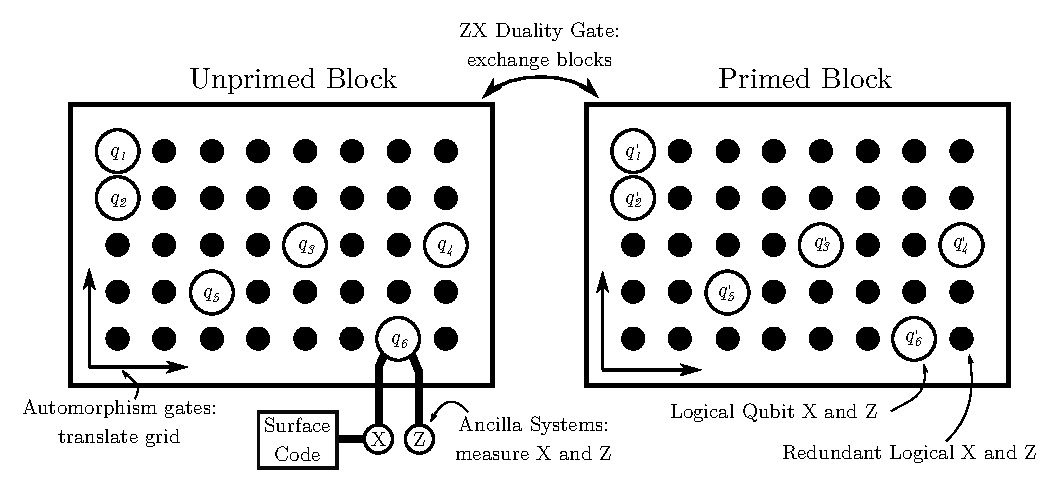
\includegraphics[height=7cm]{0808_better_conceptual.pdf}
     \caption{Conceptual diagram depicting the manner by which logical operators can be loaded into and out of a BB LDPC code. In \ssec{logical_pauli_operators} we derive that there are two blocks of logical Pauli operators corresponding to a 2d grid. Some subset of these grid elements can be chosen as logical qubits (large dots) and the other elements correspond to various Pauli products (small dots). In \ssec{automorphisms} we show that there are fault tolerant logical gates based on automorphisms that translate the grid of operators within each block, and in \ssec{ZX_duality} we give a fault tolerant gate based on a ZX-duality \cite{breuckmann2022foldtransversal} that swaps the two blocks. Finally, in \ssec{logical_measurements} we show that there exists an ancilla system based on \cite{cohen2022lowoverhead} that can measure one logical $X$ operator. We can think of this system as a probe that can access one logical qubit. Together, these operations allow external access of every logical qubit and many of their products.} 
	  
  \label{fig:ops_summary}
\end{figure}

A conceptual representation of the logical operators is shown in \fig{ops_summary}. We first derive logical Pauli operators for BB LDPC codes, and find that the logical qubits divide into an ``unprimed'' and a ``primed'' block with equal size and symmetrical structure. We visualize the primed and unprimed block as two sheets featuring a 2D grid of logical operators. Some of these grid cells contain one of the $k/2$ logical qubits per sheet. 


Next, we show that there exists a set of fault tolerant depth-four circuits that implement a small family of commuting logical $\cnotgate$ circuits. These gates are based on automorphisms of the code: permutations of the data qubits that commute with the stabilizer. Based on their group structure we can think of the automorphism gates as translations of a 2D grid of operators within each of the primed and unprimed blocks. Furthermore, we follow  \cite{breuckmann2022foldtransversal} to derive a fault tolerant operation based on a ZX-duality that also allows us to swap the two blocks while also applying Hadamard gates to all qubits.





Finally, we show how to leverage techniques from \cite{cohen2022lowoverhead} to extend the Tanner graph to a larger Tanner graph allowing fault-tolerant measurement of one logical $X$ and one logical $Z$ operator. Various subgraphs of this extended Tanner graph contain either this logical $X$ or $Z$ operator as a stabilizer. This construction acts as a ``probe'' that gives us access to one of the logical qubits. 

Measurements of both logical $X$ and $Z$ operators on any qubit can be realized by conjugating this measurement by gates based on automorphisms and the ZX-duality. We can think of this as shifting any desired qubit to be the target of the probe using translation and exchange of the two blocks.

Logical $X$ and $Z$ measurement of any logical qubit also enables transfer of data into and out of the code using a teleportation circuit. This teleportation can be realized through a product measurement of the logical Pauli in the BB code, and a logical Pauli in another quantum error correction code. While the Tanner graph of the BB code demands thickness-2, we show how the ancilla system corresponding to the logical $X$ measurement can be implemented in an ``effectively planar'' Tanner graph. This makes it possible two connect this ancilla system to another quantum error correction code, like a surface code, within a thickness-2 implementation. This capability indicates the suitability of BB LDPC codes as a fault tolerant quantum memory.

\edit{On the other hand, this construction incurs rather significant resource overhead that undercuts the compactness of the error correction codes introduced in this paper. For example, to equip the $[[144,12,12]]$ code with ancilla systems capable of measuring $X$ and $Z$, we require $2 \,{\times}\, 30 \,{\times}\, (2d{-}1) = 1380$ additional qubits on top of the original 288. However, the argument for fault-tolerance from \cite{cohen2022lowoverhead} is designed to be very broadly applicable, and hence may demand excessively many resources for any particular error correction code. We consider it very likely that the size of these systems can be significantly reduced. We leave resource optimization of this scheme for future work.}

\subsection{Logical Pauli Operators}
\label{ssec:logical_pauli_operators}

In this section we derive that the logical Pauli matrices of BB LDPC codes split into a ``primed'' and an ``unprimed'' block with $|\mathcal{M}| = \ell m$ many $X$ operators and $Z$ operators each. Operators in the primed block commute with operators in the unprimed block, and the two blocks have identical commutation structure.

We begin by introducing some new notation for Pauli matrices acting on the data qubits. We denote with $\mathbb{F}_2^{\mathcal{M}}$ the set of polynomials over $\mathbb{F}_2$ with monomials from $\mathcal{M}$. This is equivalent to the quotient ring obtained from $\mathbb{F}_2[x,y]$ by identifying $x^\ell= y^m = 1$. With $x = S_m\otimes I$ and $y = I \otimes S_\ell$, the elements of $\mathbb{F}_2^{\mathcal{M}}$ have natural matrix representations, and can also be interpreted as sets since the coefficient on any particular $x \in \mathcal{M}$ is either 0 or 1.


For $P,Q \in \mathbb{F}_2^{\mathcal{M}}$, we can consider the set of qubits $q(L,\alpha)$ for $\alpha \in P$ and $q(R,\beta)$ for $\beta \in Q$.   We write $X(P,Q)$ to denote a Pauli matrix acting as $X$ on this collection of qubits, and identity elsewhere. Similarly, $Z(P,Q)$ denotes $Z$ acting on $q(L,\alpha)$ for $\alpha \in P$ and $q(R,\beta)$ for $\beta \in Q$. For example, we can recall that $q(L,\beta)$ is connected to $q(X,\alpha)$ whenever $\beta \in A\alpha$, and see that the stabilizer corresponding to $q(X,\alpha)$ becomes $X(\alpha A, \alpha B)$. Similarly, the stabilizer corresponding to $q(Z,\alpha)$ can be written as $Z(\alpha B^T,\alpha A^T)$. There is also the following useful fact:

\begin{lemma} $X(P,Q)$ anticommutes with $Z(\bar P,\bar Q)$ if and only if $1 \in P\bar P^T + Q\bar Q^T$.
\end{lemma}
%SBB: I've added a proof. This might help the reader to understand the monomial notations better. PR: Looks great, thank you!
\begin{proof}
Write 
\[
P=\sum_{\alpha\in \calM} p_\alpha \alpha,
\quad 
\bar{P}=\sum_{\alpha\in \calM} \bar{p}_\alpha \alpha,
\quad
Q=\sum_{\alpha\in \calM} q_\alpha \alpha,
\quad
\bar{Q}=\sum_{\alpha\in \calM} \bar{q}_\alpha \alpha,
\]
where  $p_\alpha,\bar{p}_\alpha,q_\alpha,\bar{q}_\alpha\in \FF_2$ are coefficients.
Pauli operators $X(P,Q)$ and $Z(\bar{P},\bar{Q})$ overlap on a qubit
$q(L,\alpha)$  iff $p_\alpha \bar{p}_\alpha=1$
and overlap on a qubit $q(R,\alpha)$ iff $q_\alpha\bar{q}_\alpha=1$.
Thus  $X(P,Q)$ and $Z(\bar{P},\bar{Q})$ anti-commute
iff  $\sum_{\alpha \in \calM} p_\alpha \bar{p}_\alpha + q_\alpha \bar{q}_\alpha$
is odd. 
We have 
\[
P\bar{P}^T = \sum_{\alpha \in \calM} p_\alpha \bar{p}_\alpha 1 + \ldots
\quad \mbox{and} \quad
Q\bar{Q}^T =  \sum_{\alpha \in \calM} q_\alpha \bar{q}_\alpha 1 + \ldots
\]
where dots represent all monomials different from $1$. By linearity,
\[
P\bar{P}^T + Q\bar{Q}^T
=\sum_{\alpha \in \calM}
(p_\alpha \bar{p}_\alpha
+q_\alpha \bar{q}_\alpha)1+\ldots.
\]
Thus $X(P,Q)$ and $Z(\bar{P},\bar{Q})$ anti-commute
iff $P\bar{P}^T + Q\bar{Q}^T$ contains the monomial $1$.
\end{proof}


Without loss of generality, we can express logical Pauli matrices as either $X(P,Q)$ or $Z(Q^T, P^T)$ via a choice of $P,Q \in \mathbb{F}_2^{\mathcal{M}}$. The operator $X(P,Q)$ commutes with the stabilizer $Z(\alpha B^T, \alpha A^T)$ whenever $1 \not\in P(\alpha B^T)^T + Q (\alpha A^T)^T = \alpha^T (PB + QA) $. This is equivalent to $\alpha \not\in PB + QA$. Since we must have $\alpha \not\in PB + QA$ for all $\alpha$, we see that $X(P,Q)$ commutes with the stabilizer whenever $PB + QA$ vanishes. Similarly we can derive that $Z(Q^T, P^T)$ commutes with the stabilizer when $PB + QA = 0$. 

We aim to construct a family of solutions to $PB + QA = 0$ which give rise to a basis of logical qubits defined by a set of operators $\{\bar X_1, \bar X_2, ..., \bar Z_1, \bar Z_2, ... \}$ with the correct commutation relations.  To do so, let us make some observations about Pauli operators defined via solutions to $PB + QA = 0$. First, if $P,Q$ are a solution, then so are $\alpha P, \alpha Q$ for any $\alpha \in \mathcal{M}$, so each $P,Q$ immediately gives rise to a family of $|\mathcal{M}| = lm$ logical operators for both $X$ and $Z$. Second, consider using the same $P,Q$ to define both $X(\alpha P, \alpha Q)$  and $Z(\beta Q^T, \beta P^T)$. Then these operators always commute because $\beta \alpha^T \in PQ + QP = 0$ never holds. So we require at least two solutions to $PB+QA = 0$ to define a set of operators with nontrivial commutation relations. 

For reasons described later in \ssec{logical_measurements}, we would like a logical $X$ operator with no support on $q(R)$. To this end, we select $f,g,h \in \mathbb{F}_2^{\mathcal{M}}$ that satisfy $Bf = 0$ and $gB + hA = 0$, yielding two solutions to the equation $PB+QA = 0$ with $P,Q = f,0$ and $P,Q = g,h$. These yield the following family of logical operators for all $\alpha \in \mathcal{M}$:
\begin{equation}
\begin{aligned}
	 \bar X_\alpha &:= X(\alpha f,0) \hspace{1.2cm} \bar Z_\alpha := Z(\alpha h^T, \alpha g^T)\\
    \bar X'_\alpha &:= X(\alpha  g, \alpha  h) \hspace{1cm} \bar Z'_\alpha := Z(0, \alpha f^T) 
\end{aligned}\label{eq:logicalpaulis}
\end{equation}

For all $\alpha,\beta $, we see that $\bar X_\alpha, \bar Z'_\beta$ always commute because $f0^T + 0f^T = 0$, and $\bar X'_\beta,\bar Z_\alpha$ always commute because $gh+hg=0$. Furthermore, $\bar X_\alpha, \bar Z_\beta$ and $\bar X'_\alpha, \bar Z'_\beta$ form anticommuting pairs when $\alpha^T\beta \in fh$. We see that we have constructed two independent blocks of logical operators with symmetrical structure. It follows that each of these blocks must contain a set of operators that define $k/2$ qubits. We name these the ``unprimed'' and ``primed'' logical blocks with $\bar X_\alpha, \bar Z_\beta$ and $\bar X'_\alpha, \bar Z'_\beta$ respectively.

Not all choices of $f,g,h$ span all $k$ logical qubits, but valid choices are readily enumerated in software. Solutions to $Bf = 0$ and $gB + hA = 0$ correspond to null spaces of $B$ and $\begin{bmatrix}B \\ A\end{bmatrix}$ respectively, which can be constructed by Gaussian elimination. Gaussian elimination can also be used to check if the operators $\bar X_\alpha, \bar Z_\alpha, \bar X'_\alpha, \bar Z'_\alpha$ together span $k$ qubits up to the stabilizer. We find all codes in \ifmain{\tab{codes}}{Table~\tabcodes in the main text} admit several such choices of $f,g,h$. In \tab{f_polys} we show a particularly favorable choice of $f,g,h$ for the $[[144,12,12]]$ code where the resulting logical operators have minimum weight.

%SBB: perhaps we should clarify what do we mean by the weight of a polynomial.  PR: or we could just refer to the weight of X(f,0) instead. % PR: Yup!


To identify logical qubits we can enumerate choices of monomials $\{n_1, n_2, \ldots,n_{k/2}\}$ and $\{m_1, m_2, \ldots,m_{k/2}\}$ such that $n_i^T m_j \in fh$ exactly when $i = j$.  That way, $\bar X_{n_i}, \bar Z_{m_i}$ as well as $\bar X'_{n_i}, \bar Z'_{m_i}$  for $i = 1...k/2$ form a set of $k$ logical qubits: $\bar X_{n_i}$ anticommutes with $\bar Z_{m_j}$ exactly when $i = j$. A brute force search readily finds choices of $\{n_i\},\{m_i\}$.


\begin{table}
	\begin{center}
\begin{tabular}{|c|c|c|}
	\multicolumn{3}{c}{Polynomials for Logical Pauli Matrices in the $[[144,12,12]]$ Code}\\[2mm]\hline
	$f$ & $g$ & $h$ \\ \hline
	\resizebox{0.3\textwidth}{!}{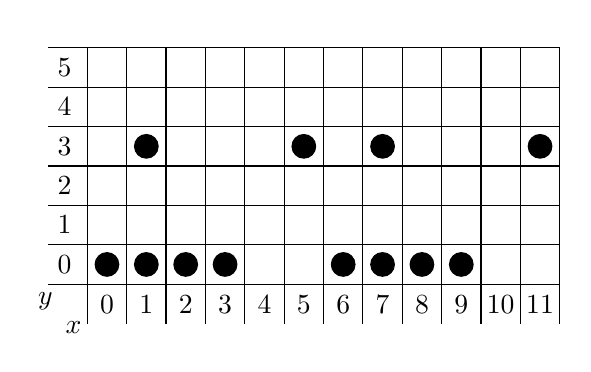
\begin{tikzpicture}
			\draw (-0.4,-0.75) node[anchor=south west] {$x$};
			\draw (-0.75,-0.45) node[anchor=south west] {$y$};
			\foreach \x in { -1,0,1,2,3,4,5,6,7,8,9,10,11 }
			\draw (\x / 2 + 0.5,-0.5) -- (\x / 2 + 0.5,3.0);
			\foreach \x in { 0,1,2,3,4,5,6,7,8,9,10,11 }
			\draw (\x / 2 + 0.25,-0.5) node[anchor=south] { \x };
			\foreach \y in { -1,0,1,2,3,4,5 }
			\draw (-0.5, \y / 2 + 0.5) -- (6.0, \y / 2 + 0.5);
			\foreach \y in { 0,1,2,3,4,5 }
			\draw (-0.5, \y / 2 + 0.25) node[anchor=west] { \y };
			\foreach \x / \y in { 1 / 0,0 / 0,2 / 0,3 / 0,6 / 0,7 / 0,8 / 0,9 / 0,1 / 3,5 / 3,7 / 3,11 / 3 }
			\draw[fill=black] (\x / 2 + 0.25,\y / 2 + 0.25) circle (0.15);
			\draw[transparent] (-0.5, 3.25) -- (6.0,3.25);
	\end{tikzpicture}}  & \resizebox{0.3\textwidth}{!}{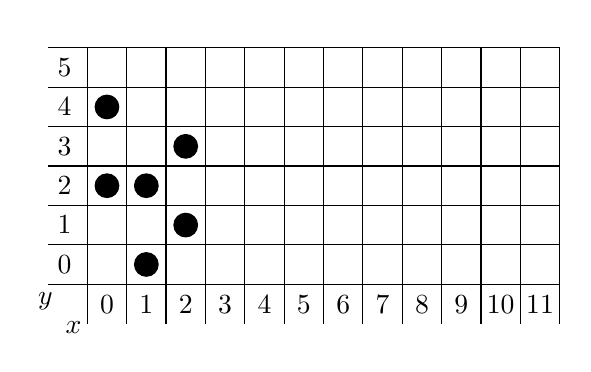
\begin{tikzpicture}
			\draw (-0.4,-0.75) node[anchor=south west] {$x$};
			\draw (-0.75,-0.45) node[anchor=south west] {$y$};
			\foreach \x in { -1,0,1,2,3,4,5,6,7,8,9,10,11 }
			\draw (\x / 2 + 0.5,-0.5) -- (\x / 2 + 0.5,3.0);
			\foreach \x in { 0,1,2,3,4,5,6,7,8,9,10,11 }
			\draw (\x / 2 + 0.25,-0.5) node[anchor=south] { \x };
			\foreach \y in { -1,0,1,2,3,4,5 }
			\draw (-0.5, \y / 2 + 0.5) -- (6.0, \y / 2 + 0.5);
			\foreach \y in { 0,1,2,3,4,5 }
			\draw (-0.5, \y / 2 + 0.25) node[anchor=west] { \y };
			\foreach \x / \y in { 1 / 2,0 / 4,2 / 3,1 / 0,0 / 2,2 / 1 }
			\draw[fill=black] (\x / 2 + 0.25,\y / 2 + 0.25) circle (0.15);
			\draw[transparent] (-0.5, 3.25) -- (6.0,3.25);
	\end{tikzpicture}}  & \resizebox{0.3\textwidth}{!}{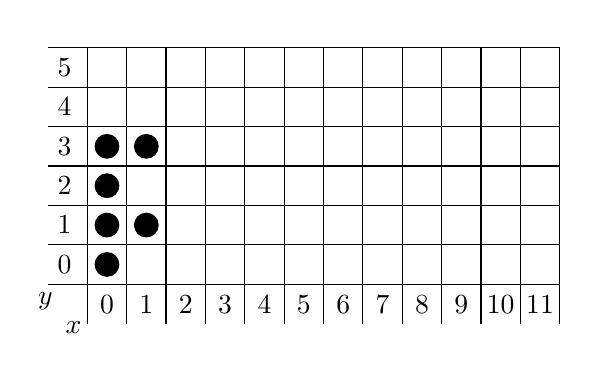
\begin{tikzpicture}
			\draw (-0.4,-0.75) node[anchor=south west] {$x$};
			\draw (-0.75,-0.45) node[anchor=south west] {$y$};
			\foreach \x in { -1,0,1,2,3,4,5,6,7,8,9,10,11 }
			\draw (\x / 2 + 0.5,-0.5) -- (\x / 2 + 0.5,3.0);
			\foreach \x in { 0,1,2,3,4,5,6,7,8,9,10,11 }
			\draw (\x / 2 + 0.25,-0.5) node[anchor=south] { \x };
			\foreach \y in { -1,0,1,2,3,4,5 }
			\draw (-0.5, \y / 2 + 0.5) -- (6.0, \y / 2 + 0.5);
			\foreach \y in { 0,1,2,3,4,5 }
			\draw (-0.5, \y / 2 + 0.25) node[anchor=west] { \y };
			\foreach \x / \y in { 0 / 3,0 / 2,1 / 3,0 / 1,0 / 0,1 / 1 }
			\draw[fill=black] (\x / 2 + 0.25,\y / 2 + 0.25) circle (0.15);
			\draw[transparent] (-0.5, 3.25) -- (6.0,3.25);
	\end{tikzpicture}}   \\ \hline
	\multicolumn{3}{c}{}\\
\end{tabular}
	\end{center}
	\caption{\label{table:f_polys} Choices of polynomials $f,g,h$ such that $\bar X_\alpha := X(\alpha f,0)$ and $\bar Z_\alpha = Z(\alpha h^T, \alpha g^T)$ as defined in equation \ref{eq:logicalpaulis} are minimum-weight logical Pauli operators. The dots represent the monomials of the form $x^iy^j$ with coefficient 1.  If we let $\{n_i\} = \{1, y, x^2y, x^2y^5, x^3y^2, x^4\}$ and $\{m_i\} = \{ y, y^5, xy, 1, x^4, x^5y^2 \}$, then $\bar X_{n_i},\bar Z_{m_j}$ anticommute exactly when $i = j$. When used to construct an ancilla system as in Section~\ref{ssec:logical_measurements}, these polynomials give a system with 60 qubits per layer.
	} 
\end{table}
%SBB: what is the meaning of "Cost" in this table ? I guess the cost has something to do with the size of the ancilla system. PR: Ah, I described in the main text but it looks like I forgot to describe it in the table caption.

\subsection{Logical Gates based on Automorphisms}
\label{ssec:automorphisms}

An automorphism of an error correction code is a permutation of the physical qubits that is equivalent to a permutation of the checks 
%SBB: added a comment. PR: Yes, this works. We could also say "a permutation of the  ... that commutes with the stabilizer." Maybe that's simpler?
(more generally, an automorphism can map a check operator to a product of check operators).  
We focus on permutations that are implementable using fault tolerant circuits within the connectivity already required for syndrome measurements.

The existing connectivity admits some natural fault tolerant circuits implementing a particular family of permutations on the data qubits. BB LDPC codes feature two data registers $q(L),q(R)$ and two
%SBB: perhaps we should use the term "check register" instead of "ancillary register" for consistency with other sections. PR: agreed.
check registers $q(X),q(Z)$. We consider circuits that transfer the qubits from the data registers to the ancilla registers, and back again on a different path. The adjacency matrices describing the connectivity between the data and the ancilla registers are given by $A$ and $B$, which are the sum of three monomials $A_1, A_2, A_3$ and $B_1,B_2,B_3$ in $\mathcal{M}$. Each monomial is a permutation and thus describes a vertex-disjoint set of edges between the data and ancilla block. Hence, all swaps along these edges can be parallelized.
In a single circuit we can either swap along the edges defined by $A$ which are $q(L)\leftrightarrow q(X)$ and $q(R)\leftrightarrow q(Z)$, or along edges defined by $B$ which are $q(L)\leftrightarrow q(Z)$ and $q(R)\leftrightarrow q(X)$. See also \ifmain{\fig{navigation} A)}{Figure~\fignavigation A) in the main text}. 
%SBB: Figure 5C does not exist, as far as I can tell. PR: Fixed.

The monomial defining the particular set of edges in each of these sets of swaps can be chosen independently for each stage of the permutation (data $\to$ ancilla or ancilla $\to$ data), and on each side of the Tanner graph. 
 %SBB: if I understand correctly, we can go from q(L) to q(X) by applying A_j^T and then go from q(X) to q(L) by applying A_k. I don't see how to get from q(L) to q(X) by applying A_j. PR: Yes, some transposes were missing.
For example, we can select any $A_j, A_k, A_{j'}, A_{k'}$ and move $q(L) \to_{A_j^T} q(X) \to_{A_{k}} q(L)$ and simultaneously move $q(R) \to_{A_{k'}} q(Z) \to_{A_{j'}^T} q(R)$. However, we will see later that it is necessary to select $A_j = A_{j'}$ and $A_k = A_{k'}$. Furthermore, these swaps admit a standard optimization: if we initialize the check registers $q(X),q(Z)$ to the $|0\rangle$ state, then circuits implementing these permutations have $\cnotgate$ depth four. If we also reset qubits to the $|0\rangle$ state in between the swaps wherever possible, we obtain circuits whose errors cannot propagate between physical qubits, and are hence fault tolerant. See \tab{automorphisms}.

 
We now verify that the permutations implemented by the circuits described above are indeed automorphisms. After having applied an `A' type permutation based on $A_j,A_k$, the qubits are permuted by $q(L, \alpha) \leftrightarrow q(L,A^T_k A_j \alpha )$ and $q(R, \alpha) \leftrightarrow q(R,A^T_{k}A_{j}\alpha )$. We see that this transforms a Pauli matrix by $X(P,Q) \to X( A_j A_k^T P, A_j A_k^T Q  )$. Consequently, the stabilizers are transformed as $X(\alpha A, \alpha B) \to X(\alpha  A_j A_k^T A, \alpha A_j A_k^T B  )$, which is the same as permuting the $X$ checks by $\alpha \to \alpha A_j A_k^T$. The $Z$ stabilizers are also permuted by $\alpha \to \alpha A_j A_k^T$, so the described circuit indeed implements an automorphism. Notice also that this only works because the $q(L)$ and $q(R)$ blocks were transformed by the same $A_j A_k^T$. The `B' type permutations can be verified to be automorphisms in the same manner, permuting the checks by some $B_jB_k^T$.

These automorphisms allow us to fault tolerantly implement a subgroup of the Clifford gates. As we saw in \ifmain{\lem{connected}}{Lemma~\lemconnected in the main text}, shifts of the form $A_j A_k^T$ or $B_jB_k^T$ generate the entire group $\mathcal{M}$ whenever the Tanner graph is connected.
%SBB: I don't think we can implement all permutations in M. We can only implement shifts by x and y. Note that there are (ell m)! permutations of M and there are only ell m shifts. PR: Yes, the we cannot implement arbitrary permutations of M - we can only implement a group of permutations congruent to M. Maybe I can make this more clear....
Therefore, by leveraging these permutations as generators, we can perform all translations of the tori containing $q(L), q(R)$ using fault tolerant circuits of varying depth. An automorphism defined by an element $s \in \mathcal{M}$ transforms $\bar X_{n_i} \to \bar X_{sn_i}$, $\bar Z_{m_i} \to \bar Z_{sm_i}$ and similarly for the primed logical Pauli matrices.  This capability is critical for addressing all logical qubits.

We can also comment on the nature of these operations as logical gates, although they are less useful in this sense. There is one such operation per element in $\mathcal{M}$, and since $\mathcal{M}$ is Abelian the subgroup of Clifford gates implemented by these automorphisms must be Abelian as well.  A transformation of this form cannot act like the logical identity so all of these gates (except $s= 1$) are nontrivial. Since automorphism operations take $\bar X$ to $\bar X$ and $\bar Z$ to $\bar Z$, and they must hence be logical $\cnotgate$ circuits up to a logical Pauli correction. While it is not clear how to use these $\cnotgate$ circuits to facilitate useful computations, they may make for interesting test cases in an implementation.

\begin{table}[t]
\begin{center}
\begin{tabular}{cc}
\multicolumn{2}{c}{`A' type automorphism based on any $A_j,A_k$}\\
{\centering
\begin{minipage}{7cm}
	\begin{algorithmic}
	\State{}
	\For{$\alpha \in \mathcal{M}$}
	\State{$\initZ{q(X,\alpha)}$}
	\State{$\cnot{q(L,A_j\alpha )}{q(X,\alpha)}$}
	\State{$\cnot{q(X,\alpha)}{q(L,A_j\alpha)}$}
	\State{$\initZ{q(L,A_k^T\alpha)}$}
	\State{$\cnot{q(X,\alpha)}{q(L,A_k\alpha)}$}
	\State{$\cnot{q(L,A_k\alpha)}{q(X,\alpha)}$}
	\EndFor
	\State{}
	\end{algorithmic}
\end{minipage}}
&
{\centering
\begin{minipage}{7cm}
	\begin{algorithmic}
	\State{}
	\For{$\alpha \in \mathcal{M}$}
	\State{$\initZ{q(Z,\alpha)}$}
	\State{$\cnot{q(R,\alpha)}{q(Z,A_{j}\alpha)}$}
	\State{$\cnot{q(Z,A_{j}\alpha)}{q(R,\alpha)}$}
	\State{$\initZ{q(R,A_k\alpha)}$}
	\State{$\cnot{q(Z,A_{k}\alpha)}{q(R,\alpha)}$}
	\State{$\cnot{q(R,\alpha)}{q(Z,A_{k}\alpha)}$}
	\EndFor
	\State{}
	\end{algorithmic}
\end{minipage}}
 \\ \hline \\
 \multicolumn{2}{c}{`B' type automorphism based on any $B_j,B_k$}\\
{\centering
\begin{minipage}{7cm}
	\begin{algorithmic}
	\State{}
	\For{$\alpha \in \mathcal{M}$}
	\State{$\initZ{q(X,\alpha)}$}
	\State{$\cnot{q(R,B_j\alpha)}{q(X,\alpha)}$}
	\State{$\cnot{q(X,\alpha)}{q(R,B_j\alpha)}$}
	\State{$\initZ{q(R,B^T_k\alpha)}$}
	\State{$\cnot{q(X,\alpha)}{q(R,B_k\alpha)}$}
	\State{$\cnot{q(R,B_k\alpha)}{q(X,\alpha)}$}
	\EndFor
	\State{}
	\end{algorithmic}
\end{minipage}}
&
{\centering
\begin{minipage}{7cm}
	\begin{algorithmic}
	\State{}
	\For{$\alpha \in \mathcal{M}$}
	\State{$\initZ{q(Z,\alpha)}$}
	\State{$\cnot{q(L,\alpha)}{q(Z,B_{j}\alpha)}$}
	\State{$\cnot{q(Z,B_{j}\alpha)}{q(L,\alpha)}$}
	\State{$\initZ{q(L,B_k\alpha)}$}
	\State{$\cnot{q(Z,B_{k}\alpha)}{q(L,\alpha)}$}
	\State{$\cnot{q(L,\alpha)}{q(Z,B_{k}\alpha)}$}
	\EndFor
	\State{}
	\end{algorithmic}
\end{minipage}}
 \\ 
\end{tabular}
\end{center}
\caption{\label{table:automorphisms} Circuits implementing automorphisms of a BB LDPC code within the connectivity already present for syndrome checks. These circuits are fault tolerant and have $\cnotgate$ depth four. If $s = A_j A_k^T$ or $s = B_j B_k^T$, then the logical gate implemented by these automorphisms performs the transformation $\bar X_\alpha, \bar Z_\alpha, \bar X'_\alpha, \bar Z'_\alpha \to \bar X_{s\alpha}, \bar Z_{s\alpha}, \bar X'_{s\alpha}, \bar Z'_{s\alpha}$.}
\end{table}
%SBB: I am not sure if these circuits are correct. For example, the first CNOT in the top left panel does not appear to be compatible with the Tanner graph. We have an edge between q(X,alpha) and q(L,A_j alpha), as discussed in the second paragraph of section 8.1. However, we don't have an edge between q(X,alpha) and q(L,A_j^T alpha). PR: Yes, everything was transposed. This was probably because of the convention switching...

\subsection{Accessing the Primed Block via a ZX-duality}
\label{ssec:ZX_duality}
 
%SBB: perhaps we can change "stabilizer" to "check" in this sentence for consistency. PR: Yup! Also made the definition a bit more general
A ZX-duality is a permutation of the logical qubits that commutes with the stabilizer, except that it turns $X$ checks into $Z$ checks and $Z$ checks into $X$ checks. A physical circuit implementing this permutation and then applying Hadamard to all data qubits always acts as a logical gate \cite{breuckmann2022foldtransversal}. In this section we focus on the implementation of a particular ZX-duality with applications for readout. We leave discovery and implementation of other ZX-dualities for future work. In particular, we derive a general method for constructing fault tolerant circuits for implementing a particular ZX-duality that is present in all BB LDPC codes. While the circuits from this construction are generally quite expensive, they may be amenable to further optimization and can be used sparingly in practice.


Consider a permutation of data qubits that swaps $q(L,\alpha)$ with $q(R,\alpha^{T})$ for all $\alpha \in \mathcal{M}$. A check qubit $q(X,\beta)$ which previously implemented the stabilizer $X(\beta A, \beta B )$ now is connected to the qubits $q(L, (\beta B)^T)$ and $q(R,(\beta A)^T)$ instead, corresponding to the check $Z(\beta^T B^T , \beta^T A^T)$. We see that this permutation switches the stabilizer implemented by $q(X,\beta)$ with the stabilizer implemented by $q(Z,\beta^T)$, so this permutation is indeed a ZX-duality.

We can also see that implementing this permutation and applying Hadamard to all qubits takes logical Pauli matrices to logical Pauli matrices. In particular, the operation swaps $\bar X_\alpha = X(\alpha f,0)$ with $\bar Z'_{\alpha^T} = Z(0,\alpha^T f^T)$, as well as $\bar Z_\alpha = Z(\alpha h^T, \alpha g^T)$ with $\bar X'_{\alpha^T} := X(\alpha^T g, \alpha^T h)$. This operation swaps the primed and unprimed logical blocks, transposes the grid of operators, and applies logical Hadamard to all qubits. Since we can measure logical $X$ for all qubits in the unprimed block using the ancilla system described in \ssec{logical_measurements}, we can use this operation to measure logical $Z$ for qubits in the primed block.

For the rest of this section we describe a fault tolerant method for implementing this operation. We begin with exchanging $q(L)$ and $q(R)$: since these blocks are connected by pairs of edges in $q(X)$ and $q(Z)$, for any $A_i \in A$ and $B_j \in B$ there exists a loop connecting the qubits $q(L,\alpha) \to q(X,A_i^T \alpha) \to q(R, B_j A_i^T \alpha) \to q(Z, B_j \alpha) \to q(L,\alpha)$.
A circuit identical in shape to those in \tab{automorphisms} hence performs a fault tolerant exchange of $q(L,\alpha)$ and $q(R, B_j A_i^T\alpha)$ for all $\alpha$. The additional shift of $B_j A_i^T$ can be removed via an additional automorphism gate. It remains to exchange $q(L,\alpha) \leftrightarrow q(L,\alpha^T)$, as well as $q(R,\alpha)\leftrightarrow q(R,\alpha^T)$ for all $\alpha$, which is significantly more complicated. We focus on $q(L,\alpha) \leftrightarrow q(L,\alpha^T)$ in our discussion but it will be clear the exact same transformations are implementable on $q(R)$ in parallel with those on $q(L)$.

\begin{figure}[t]
  \centering
    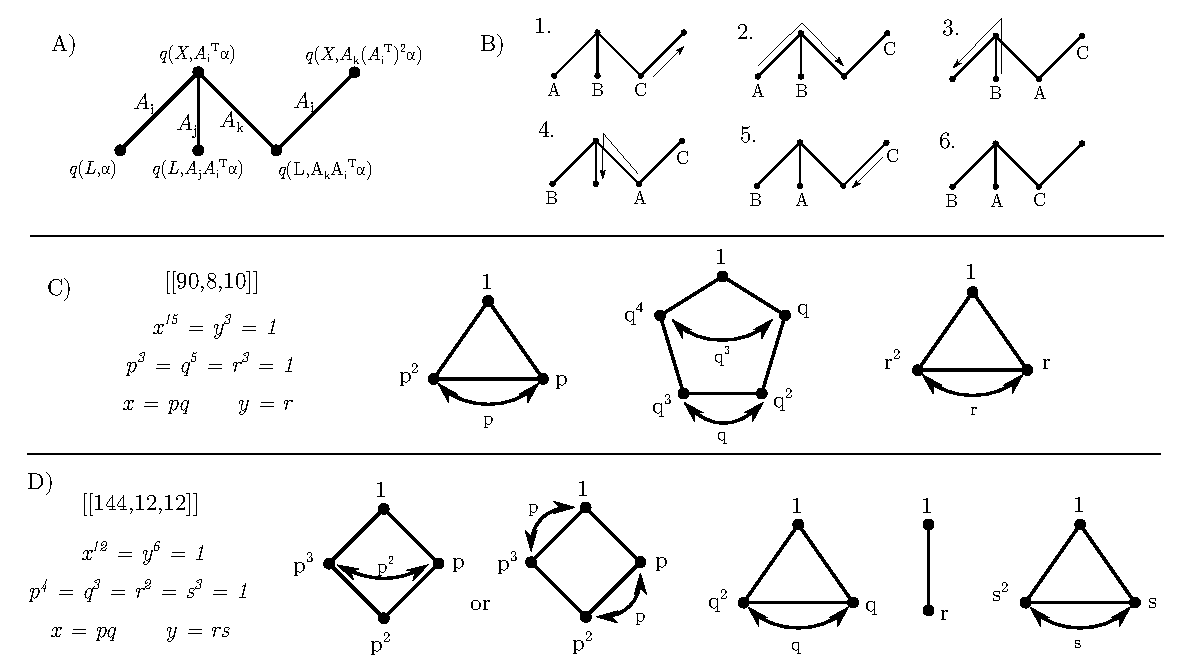
\includegraphics[height=8cm]{duality_implementation.pdf}
     \caption{Diagrams for the description of the implementation of the ZX-duality permutation. A) A subgraph of the Tanner graph providing enough connectivity to fault tolerantly swap $q(L,\alpha)$ and $q(L,A_j A_i^T\alpha)$. B) A sequence of shifts of the data on the qubits in the $q(L)$ block that performs the desired exchange without interacting qubits directly. A naive implementation of this sequence has $\cnotgate$ depth 12. C) D) Decomposition of the generators of $\mathcal{M}$ via the classification of finite Abelian groups for two different codes. Drawing the Cayley graph of the subgroup for each generator reveals the ratios defining pairs of qubits that must be exchanged to implement the permutation $q(L,\alpha) \leftrightarrow q(L,\alpha^T)$.}
  \label{fig:duality_implementation}
\end{figure}
%SBB: I was confused by panel A). Based on the definition in the second paragraph of section 8.1, the Tanner graph has an edge between q(X,alpha) and q(L,A_j alpha). However there is no edge between q(X,A_j alpha) and q(L,alpha). PR: Yes, somehow I had everything transposed again. Should be fixed now.


Fault tolerant implementation of the permutation $q(L,\alpha) \leftrightarrow q(L,\alpha^T)$ can be achieved using a more sophisticated version of the fault tolerant circuits in \tab{automorphisms} used for implementing automorphisms. These circuits relied on the existence of a connected loop of alternating check and data qubits, enabling a short depth fault tolerant circuit implementing a cyclic permutation of the data qubits therein. The same connectivity can be leveraged to implement a fault tolerant nearest neighbor swap of two data qubits connected by a check qubit. The fault tolerance of these circuits relies on the same principle: while a swap gate acting on two qubits containing data is not fault tolerant, moving a data qubit onto a blank qubit is. \fig{duality_implementation} A) shows a subgraph of the Tanner graph consisting of several connected qubits in the $q(L)$ and $q(X)$ block, and \fig{duality_implementation} B) shows a sequence of operations where two data qubits can be exchanged without ever interacting directly. This gives us the following capability: whenever the circuits in \tab{automorphisms} can implement the cyclic permutation $q(L,\alpha)\to q(L,s\alpha )$ for all $\alpha$, there also exists a circuit that can swap $q(L,\alpha)$ and $q(L,s\alpha)$ for a particular $\alpha$. Matching circuits exist for $q(R)$, and can be implemented simultaneously.

To decompose $q(L,\alpha) \leftrightarrow q(L,\alpha^T)$ into a sequence of swaps, it will be helpful to consider the group structure of $\mathcal{M}$. Consider for example the $[[90,8,10]]$ code with $x^{15}= y^3 = 1$. 
%SBB: We should use consistent notations for the cyclic group. Cyclic group of order k is denoted $\mathbb{Z}_k$, see e.g. Definition 1 on page 13. PR: Yes, this makes sense.
Following the classification of finite Abelian groups we see that $\mathcal{M} \cong \mathbb{Z}_3 \times \mathbb{Z}_5 \times \mathbb{Z}_3$. We can re-express elements of $\mathcal{M}$ using generators $p,q,r$ with $p^3 = q^5 = r^3 =1$ where $x = pq$ and $y = r$. Transforming $\alpha$ to $\alpha^T$ amounts to decomposing $\alpha$ as $\alpha = p^i q^j r^k$ and exchanging the qubit with $\alpha^T = p^{-i} q^{-j} r^{-k}$.


This exchange $p^i q^j r^k \leftrightarrow p^{-i} q^{-j} r^{-k}$ can be split into a sequence of swaps that are implementable with the method described above using \fig{duality_implementation} A) and B). It suffices to be able to exchange for any $\alpha = q^j r^k$ the qubits $q(L,p^i \alpha) \leftrightarrow q(L,\alpha p^{-i})$, as well as for any $\alpha = p^i r^k$ the qubits $q(L,q^j \alpha) \leftrightarrow q(L,\alpha q^{-j})$, and finally for any $\alpha = p^i q^j$ the qubits $q(L,r^k \alpha) \leftrightarrow q(L,\alpha r^{-k})$. This, for any $i,j,k$, creates a sequence of qubits $q(L,p^i q^j r^k) \leftrightarrow q(L,p^{-i} q^{j} r^{k})  \leftrightarrow q(L,p^{-i} q^{-j} r^{k})  \leftrightarrow q(L,p^{-i} q^{-j} r^{-k}) $ where swaps are possible along each nearest neighbor.  This is sufficient for swapping the first and last qubit in the chain. The implementation of the individual generators like $q(L,\alpha q^i) \leftrightarrow q(L,\alpha q^{-i})$ swaps may also involve additional intermediate qubits, but this only lengthens the chain and does not prohibit implementation.


The resources required for swapping $q(L,p^i \alpha) \leftrightarrow q(L,\alpha p^{-i})$ where $p^3 = 1$ and similarly for other generators depends on the order of the generator $p$ as well as the ratios $A_iA_j^T$ that can be formed using terms $A_i,A_j \in  A$ or similar ratios from $B$. See \fig{duality_implementation} C). Plotting the Cayley graph of the cyclic subgroup spanned by $p$ immediately reveals that since $p$ is order three, only a single ratio $B_iB_j^T = p$ is needed in order to swap any qubits marked $p^1$ and $p^2$, while leaving $p^0$ qubits in place. Indeed since $B = 1 + x^2 + x^7 = 1 + p^2 q^2 + p q^2$ we can implement $p = (p^2 q^2)(p q^2)^T$ in a single layer of transforms in \fig{duality_implementation} B). 

The exchange $q(L,\alpha q^i ) \leftrightarrow q(L,\alpha q^{-i})$ with $q^5 = 1$ requires two such ratios $q$ and $q^2$, the minimal depth expression of which demands the chaining together of two such transforms each. In other codes, like the $[[144,12,12]]$ code, we encounter generators $p,q,r,s$ of order $p^4 = q^3 = r^2 = s^3 = 1$. Elements of order two like $r$ require no swaps at all, and elements of order four like $p$ can be implemented either using the ratio $p^2$ or just $p$, as shown in \fig{duality_implementation} D). Numerical searches can quickly compute the most efficient decompositions of the required swaps. We give the orders of the generators, the ratios defining the required swaps, and the number of transforms required to implement them in \tab{duality_implementations}.  

We emphasize that the swap $q(L,p^i \alpha) \leftrightarrow q(L,\alpha p^{-i})$ can be performed for all $\alpha = q^j r^k$ simultaneously in parallel. This stems from the structure of the exchange circuit in \fig{duality_implementation} B). This circuit performs the swap $q(L,\alpha) \leftrightarrow q(L,A_jA_i^T \cdot \alpha)$ while using the qubit $q(L,A_kA_i^T \cdot \alpha)$ as scratch space. However, we can simultaneously want to swap $q(L,A_kA_i^T \cdot \alpha) \leftrightarrow q(L,A_jA_i^T\cdot A_kA_i^T \cdot \alpha)$ since the first step of the exchange circuit in \fig{duality_implementation} B) is to move the data marked `A' away from the qubit holding it, just as if it were a piece of data marked `C' for a different exchange.

For clarity, we compute the total depth of the circuit for the $[[144,12,12]]$ code without any further optimization. The ratios $p,q,s$ can be implemented using two ratios each via $p = x^{-3} y \cdot y^{-2} y$,   $q = y^{-3}x^2 \cdot y^{-3}x^2$ and $s = y^{-2} y \cdot y^{-2} y$. This results in a chain $q(L,\alpha) \leftrightarrow q(L, \alpha')\leftrightarrow q(L, \alpha'') ... \leftrightarrow   q(L,\alpha^T)$ of length six (counting the number of $\leftrightarrow$s). We can swap the qubits at the ends of a chain of length $n$ using $2n{-}1$ many nearest neighbor swaps. Each swap circuit of the form \fig{duality_implementation} B) can be implemented in $\cnotgate$ depth twelve, resulting in $\cnotgate$ depth $(2\cdot 6 -1)\cdot 12 = 132$ to implement $q(L,\alpha  ) \leftrightarrow q(L,\alpha^T)$. 

%SBB: My understanding is that there is a small depth circuit that implements a swap q(L,alpha)<-->q(L,alpha^T) for any fixed alpha. Can we implement all these swaps in parallel ? If not, does it mean that we have to turn off error correction while we are done with implementing all these swaps? PR: You are correct. While I think that the swaps for each generator individually e.g. q(L,p^i q^j r^k)<-->q(L,p^-i q^j r^k) can be done in parallel for all q^j r^k, the interchanges corresponding for p, q, r cannot be parallelized. This results in a rather deep circuit with no intermediate error correction. I clarified this point in the next paragraph.


Despite its fault tolerance, the implementation of this logical operation is clearly significantly more expensive than that of the automorphisms. Since the intermediate permutations corresponding to each of the generators $p,q,r$ are not ZX dualities in general, it will not be possible in general to perform error correction during this long operation. However, the significant overhead of this operation may be worth such a large cost, since it grants us the capability of accessing the primed block of qubits, effectively doubling the storage capacity of the code. This operation can also be used significantly more sparingly than the automorphism gates, and may be amenable to additional optimization. \edit{Alternatively, additional connections and qubits beyond those necessary for the Tanner graph could be introduced to more directly implement the ZX-duality, though it is likely this will sacrifice the thickness-2 property.}


\begin{table}
	\begin{center}
		\begin{tabular}{|c|c|c|c|c|}
			\hline
			Code & Base Order & Reduced Order & Required Ratios & Swap Chain Length \\ \hline \hline
			$[[72,12,6]]$ & $x^6, y^6$ &  $p^2, q^3, r^2, s^3$ & $q,s$ & 4 \\ \hline
			$[[90,8,10]]$ & $x^{15}, y^{3}$ & $p^3, q^5, r^{3}$ & $p, q, q^2, r$ & 6 \\ \hline
			$[[108,8,10]]$ & $x^9, y^6$ &  $p^9, q^2, r^3$ & $p, p^3, p^5, p^7, r$ & 9 \\ \hline
			$[[144,12,12]]$ & $x^{12}, y^6$ & $p^4, q^3, r^2, s^3$  & $p, q, s$ & 6 \\ \hline
			$[[288,12,18]]$ & $x^{12}, y^{12}$ & $p^4, q^{3}, r^4, s^3$ & $p,q,r,s$ & 10 \\ \hline
			$[[360,12,\leq24]]$ & $x^{30}, y^{6}$ & $p^2, q^3, r^5, s^2, t^3$ & $q, ps, psr^2, psr^3, t$ & 11 \\ \hline
			 %[("E",q),("E",p*s),("E",p*s*r**2),("E",p*s*r**3),("E",t*s)])
			% $[[756,16,\leq24]]$ & $x^{21}, y^{18}$ & ... prohibitive \\ \hline
		\end{tabular}
	\end{center}
     \caption{\label{table:duality_implementations} Table deriving the steps in the circuit implementing the $q(L,\alpha) \leftrightarrow q(L,\alpha^T)$, permutation for the ZX-duality for several codes. The generators of $\mathcal{M}$ are decomposed into generators following the decomposition of finite Abelian groups. Following \fig{duality_implementation} B) and C) these generators demand a set of ratios of terms in $A$ or $B$ which define fault tolerantly implementable exchanges of qubits with corresponding labels. The result is a decomposition of $q(L,\alpha) \leftrightarrow q(L,\alpha^T)$ into a chain $q(L,\alpha) \leftrightarrow q(L, \alpha')\leftrightarrow q(L, \alpha'') \leftrightarrow ... \leftrightarrow   q(L,\alpha^T)$ with length as shown (counting the number of arrows, $\leftrightarrow$).  Note the special implementation of the ratios in the $[[360,12,\leq24]]$ code: the ratios $r^2,r^3$ are not implementable, but $psr^2, psr^3$ are. This is fine if we can also perform the $ps$ ratio on its own to remove the additional transformation on some of the qubits.}
\end{table}



\subsection{Logical Measurements}
\label{ssec:logical_measurements}


\begin{figure}[t]
  \centering
    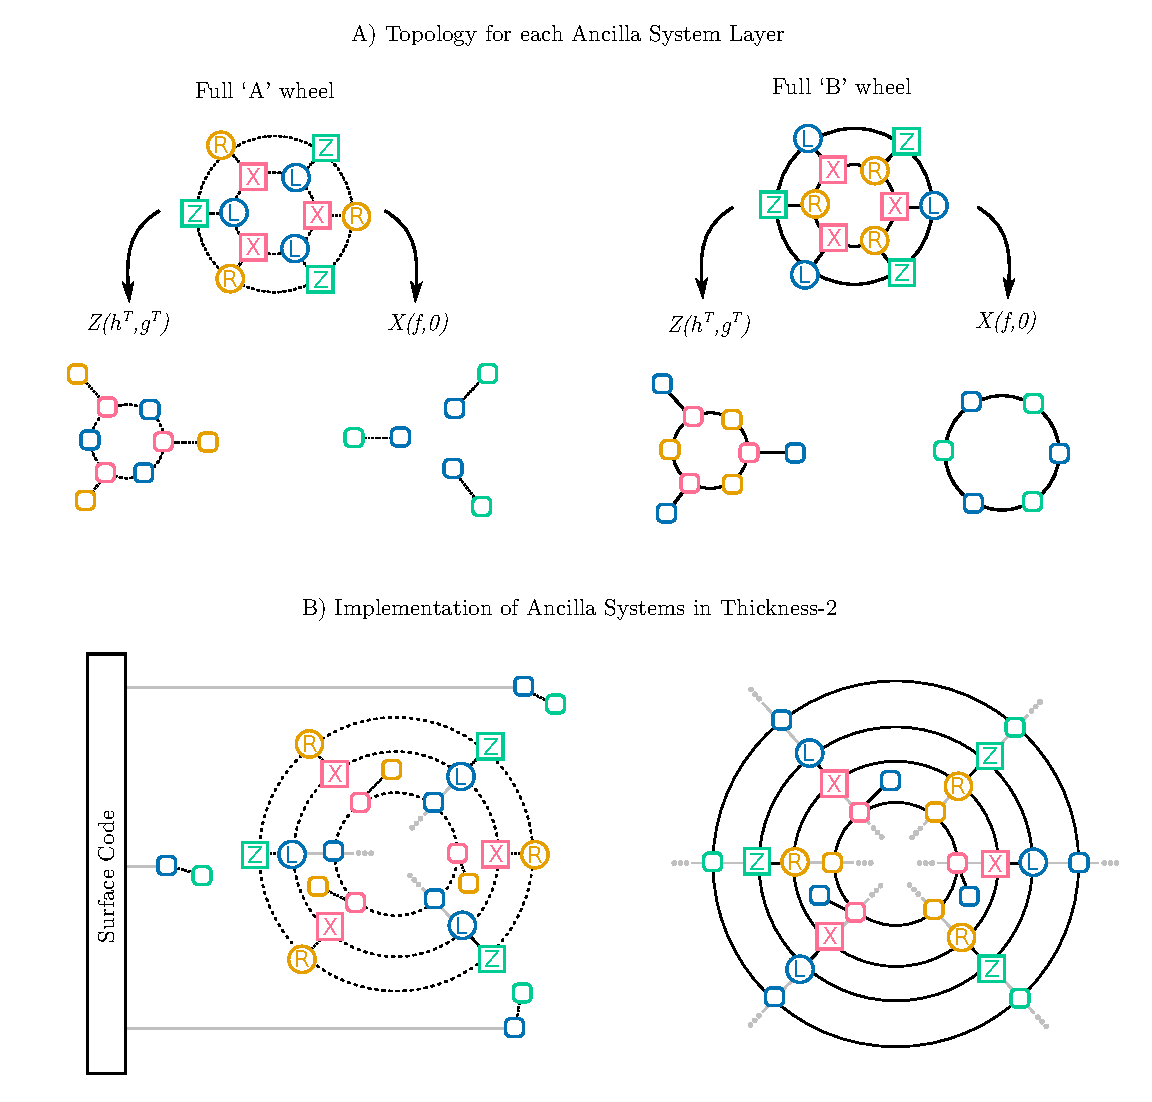
\includegraphics[width=0.9\textwidth]{dual_ancilla.pdf}
     \caption{\edit{Illustration} of the thickness-2 property of the Tanner graph of BB LDPC codes. A)  Planar embedding of each layer of the ancilla system from \ifmain{\fig{2Dlayout}~C)}{Figure~\figlayout~C) in the main text} via truncating the `A' and `B' wheels. B) Implementation of the graph from \ifmain{\fig{2Dlayout}~C)}{Figure~\figlayout~C) in the main text} within thickness-2 by nesting wheels. Wheels corresponding to $X(f,0)$ are placed on the outside and wheels corresponding to $Z(h^T,g^T)$ are placed on the inside. The $X(f,0)$ system can be connected to a surface code in the `A' plane. Here we only show one layer per system, but this construction can be repeated for arbitrarily many layers. }
	  
  \label{fig:ancilla_system}
\end{figure}


In this section we describe how to leverage methods from \cite{cohen2022lowoverhead} to implement fault-tolerant measurements of the operators $\bar X_1 = X(f,0)$ and $\bar Z_1 = Z(h^T,g^T)$. As described above, this capability suffices to measure $\bar X$ and $\bar Z$ for all logical qubits. We can also use this technique to measure various Pauli product operators by measuring $\bar X_\alpha, \bar Z_\alpha, \bar X'_\alpha, \bar Z'_\alpha$ for $\alpha$ not corresponding to logical qubits.

The measurement is facilitated by an ancilla system that extends the Tanner graph of the original code. The code defined by this extended Tanner graph contains the logical operator of interest as a stabilizer, enabling its fault tolerant measurement. A sketch of the structure of this ancilla system is given in \ifmain{\fig{2Dlayout}~C)}{Figure~\figlayout~C) in the main text}. For the logical operator $X(f,0)$, we consider a subgraph of the Tanner graph consisting of $q(L,f)$ as well as $q(Z,\alpha)$ operators corresponding to checks with support on $q(L,f)$. Similarly for the logical operator $Z(h^T, g^T)$ we consider a subgraph consisting of $q(L,h^T), q(R,g^T)$ as well as $q(X,\alpha)$ for the relevant $\alpha$. These subgraphs are copied several times and are connected together as shown in the figure: we call the resulting construction an ancilla system.  With enough copies, the code defined by the extended Tanner graph has the same distance as the original code. 

Furthermore, the ancilla system for measuring $X(f,0)$ can be connected to another quantum error correction code, such as a surface code. This enables a joint $\bar X \bar X$ measurement between a surface code qubit and any qubit within the BB code. A subsequent measurement of $Z(h^T,g^T)$ and some additional Pauli corrections then achieves a quantum teleportation circuit.

The main challenge of implementing these ancilla systems, in addition to minimizing their size, is to show that the extended Tanner graph satisfies the thickness-2 constraint. If our goal is to leverage the $X(f,0)$ ancilla system to measure a Pauli product measurement with a surface code qubit, then arguably a thickness-2 extension of the Tanner graph does not suffice since there is no obvious way of connecting it to the surface code qubit as in \ifmain{\fig{2Dlayout}~C)}{Figure~\figlayout~C) in the main text}. To this end, we show how to make the subgraph corresponding to the $X(f,0)$ ancilla system ``effectively planar'': while the graph has thickness-2, the planar graph in one plane consists entirely of connected components with two vertices. Given this property of the embedding of the $X(f,0)$ ancilla system, a connection between this system and a surface code may be facilitated by a construction that is thickness-2 overall.

An effectively planar embedding of the ancilla system relies on the fact that the logical operator $X(f,0)$ has no support on the $q(R)$ block. An implementation of more general logical operators is possible, but would require a graph that renders many ancilla qubits inaccessible from the outside. 

\edit{We briefly give a self-contained description for the construction of the ancilla system from \cite{cohen2022lowoverhead}, following their notation. Suppose we are interested in measuring a logical operator $\bar X$ that is supported on some set of qubits $V_{\bar X}$. Then, let $C_{\bar X}$ be the collection of Pauli-$Z$ checks that have support on any of the $V_{\bar X}$. If we view these as sets of vertices in a Tanner graph, and let $E_{\bar X}$ contain the edges between $V_{\bar X}$ and $C_{\bar X}$, then $\mathcal{G}_{\bar X} := (V_{\bar X},C_{\bar X}, E_{\bar X})$ forms a subgraph of the Tanner graph of the BB code.

The ancilla system is constructed out of copies of `primal layers' isomorphic to $\mathcal{G}_{\bar X}$, and `dual layers' isomorphic to $\mathcal{G}_{\bar X}^{T} := (V^T_{\bar X},C^T_{\bar X}, E^T_{\bar X})$ defined as follows: each $v \in V_{\bar X}$ has a corresponding $v^{T} \in C^{T}_{\bar X}$, each $c \in C_{\bar X}$ has a corresponding $c^{T} \in V^{T}_{\bar X}$, and each edge $(v,c) \in E_{\bar X}$ has a corresponding $(v^T,c^T) \in E^T_{\bar X}$. For some parameter $r$, the final Tanner graph is that of the BB code, plus $r$ additional copies of the dual graph labeled $\mathcal{G}_{\bar X}^{T}[j]$ for $1 \leq j \leq r$, and $r-1$ additional copies of the primal graph labeled $\mathcal{G}_{\bar X}[j]$ for $2 \leq j \leq r$. We regard the $\mathcal{G}_{\bar X}$ within the original code as $\mathcal{G}_{\bar X}[1]$. We also add additional connections between $\mathcal{G}_{\bar X}[j]$ and $\mathcal{G}_{\bar X}^T[j]$ for $j \leq r$, as well as $\mathcal{G}_{\bar X}^T[j]$ and $\mathcal{G}_{\bar X}[j+1]$ for $j < r$: specifically, we connect the associated pairs of $v,v^T$ and $c,c^T$.

It is shown by \cite{cohen2022lowoverhead} that the resulting Tanner graph defines an error correction code of distance $d$ when $r = d$. We construct two such ancilla systems: one for $\bar X := X(f,0)$ and one for $\bar Z := Z(h^T,g^T)$.} \tab{f_polys} shows a choice of $f,g,h$ for the $[[144,12,12]]$ code, defining $X(f,0)$ and $Z(h^T,g^T)$ such that these operators are all minimum weight, and define $\mathcal{G}_{\bar X}$ and $\mathcal{G}_{\bar Z}$ with 30 qubits each. \edit{To achieve $d = 12$ we hence require $2 \times 30 \times (2d-1) = 1380$ additional qubits. We suspect that significantly more efficient variations of this constructions are possible, but leave their development for future work.

The construction presented above is complicated by the fact that vertices in the Tanner graph take on alternating roles in each layer: in the primal layers the vertices $v$ are physical qubits, whereas in the dual layers the $v^T$ are checks. However, for the purposes of giving a thickness-2 decomposition we need not concern ourselves with this. If we do not distinguish between checks and physical qubits, then the primal layers $\mathcal{G}_\mathcal{X}$ and dual layers $\mathcal{G}^T_\mathcal{X}$ have isomorphic Tanner graphs.  Hence, for the purposes of the following, we view all layers as identical.

}

\edit{We now show why a} thickness-2 embedding of the $Z(h^T,g^T)$ ancilla system, and an effectively planar embedding of the $X(f,0)$ ancilla system is possible. This argument is best understood in reference to \fig{ancilla_system}. We begin by understanding the thickness-2 decomposition of each layer of the ancilla systems, leveraging \ifmain{\fig{wheel_extraction}}{Figure~\figwheelextraction in the main text}. In \fig{ancilla_system} A), we can see that \edit{$\mathcal{G}_{\bar Z}$ for} the $Z(h^T,g^T)$ system decomposes into `hairy rings' in both the `A' plane and the `B' plane since it has no support on $q(Z)$. \edit{$\mathcal{G}_{\bar X}$ for} the $X(f,0)$ system is a collection of connected pairs in the `A' plane and collection of rings in the `B' plane, since it has no support on $q(X)$.

\edit{Since $\mathcal{G}_{\bar X},\mathcal{G}_{\bar Z}$ are subgraphs of the BB code's Tanner graph, and its Tanner graph has thickness-2, and since $\mathcal{G}_{\bar X},\mathcal{G}_{\bar Z}$ and $\mathcal{G}^T_{\bar X},\mathcal{G}^T_{\bar Z}$ are isomorphic if we do not distinguish between qubits and checks, we see that each layer of the ancilla construction must be thickness-2 individually. The main challenge is to show that the connections between the layers can be facilitated without introducing any crossings.}

\fig{ancilla_system} B) shows how to connect several layers of the two ancilla systems to both the wheel graphs of the BB code, and also an ancillary surface code. We arrange the wheels of the BB code such that $q(X),q(L)$ are on the inside of the `A' wheels, and that $q(X),q(R)$ are on the inside of the `B' wheels. \edit{$\mathcal{G}_{\bar Z}$ and $\mathcal{G}^T_{\bar Z}$ for} of the $Z(h^T,g^T)$ system can be repeatedly nested inside of the wheels of the BB code. The $q(L)$ qubits can be connected together on the `A' plane, and the $q(R)$ and $q(X)$ qubits can be connected on the `B' plane. As for \edit{$\mathcal{G}_{\bar X}$  and $\mathcal{G}^T_{\bar X}$ for the} $X(f,0)$ system, the rings in the `B' plane can be wrapped around the wheels of the BB code which already allows connection of the required $q(L)$ and $q(Z)$ qubits. This leaves the pairs of connected qubits in the `A' plane completely free of any connections between the layers, making them available to be connected to a surface code system.

\edit{We have considered just two ancilla systems here for measuring $X(f,0)$ and $Z(h^T,g^T)$. However, using additional ancilla systems, especially if their size can be reduced, or equipping these two ancilla systems with additional connections to the $X(g,h)$ and $Z(0,f^T)$ logical operators are potential ways to eliminate the need for the error-prone ZX-duality from \ssec{ZX_duality} and access all logical qubits. On the other hand, it is not clear that either approach would preserve the thickness-2 property.}



\ifdefined\maindocument
\else
    \bibliographystyle{unsrt}
    \bibliography{mybib}
    \end{document}
\fi
